
% Proofchecked by Frank Nielsen, 13th-14th April 2021.
% I removed as suggested all the unnecessary \em commands when defining terms.
% Thank you very much for putting the manuscript in its final form. FN.

\documentclass[entropy,article,accept,oneauthor,pdftex,entropy]{Definitions/mdpi} 
\usepackage{amsmath,amsthm,amssymb,hyperref,cleveref,graphicx,url,rotating}


\graphicspath{{Fig/}}
 




%=================================================================
\firstpage{1} 
\makeatletter 
\setcounter{page}{\@firstpage} 
\makeatother
\pubvolume{1}
\issuenum{1}
\articlenumber{5}
\pubyear{2021}
\copyrightyear{2021}
\externaleditor{{Academic Editor: Yong Deng} 
}
\datereceived{12 March 2021} 
\dateaccepted{09 April 2021} 
\datepublished{} 
\hreflink{https://doi.org/}
%\history{Received: date; Accepted: date; Published: date}
%\updates{yes} % If there is an update available, un-comment this line


%=================================================================

\Title{On a Variational Definition for the Jensen-Shannon Symmetrization of Distances Based on the Information Radius}

\TitleCitation{On a Variational Definition for the Jensen-Shannon Symmetrization of Distances Based on the Information Radius}

\newcommand{\orcidauthorA}{0000-0001-5728-0726} 

\Author{Frank
 Nielsen \orcidA{}}
\AuthorNames{Frank Nielsen}

\AuthorCitation{Nielsen, F.}

\address[1]{ Sony Computer Science Laboratories, Tokyo 141-0022, Japan; Frank.Nielsen@acm.org}

%=================================================================




\def\calL{\mathcal{L}}
\def\calB{\mathcal{B}}
\def\calW{\mathcal{W}}
\def\Ray{\mathrm{Ray}}
\def\Exp{\mathrm{Exp}}
\def\calQ{\mathcal{Q}}
\def\Wei{\mathrm{Wei}}
\def\calV{\mathcal{V}}
\def\bbR{\mathbb{R}}
\def\Bhat{\mathrm{Bhat}}
\def\TV{\mathrm{TV}}
\def\vJS{\mathrm{vJS}}
\def\JS{\mathrm{JS}}
\def\KL{\mathrm{KL}}
\def\dmu{\mathrm{d}\mu}
\def\tr{\mathrm{tr}}
\def\calF{\mathcal{F}}
\def\calE{\mathcal{E}}
\def\calN{\mathcal{N}}
\def\calQ{\mathcal{Q}}
\def\calC{\mathcal{C}}
\def\calD{\mathcal{D}}
\def\calR{\mathcal{R}}
\def\calP{\mathcal{P}}
\def\calX{\mathcal{X}}
\def\LSE{\mathrm{LSE}}
\def\dmu{\mathrm{d}\mu}
\def\bbP{\mathbb{P}}
\def\minmax{\mathrm{minmax}}
%%%%

\abstract{We generalize the Jensen--Shannon divergence and the Jensen--Shannon diversity index by considering a variational definition with respect to a generic mean, thereby extending the notion of Sibson's information radius.
The variational definition applies to any arbitrary distance and yields a new way to define a Jensen--Shannon symmetrization of distances.
When the variational optimization is further constrained to belong to prescribed families of probability measures, we get relative Jensen--Shannon divergences and their equivalent Jensen--Shannon symmetrizations of distances that generalize the concept of information projections. Finally, we touch upon applications of these variational Jensen--Shannon divergences and diversity indices to clustering and quantization tasks of probability measures, including statistical mixtures.
}

% Keywords
\keyword{Jensen--Shannon divergence;   diversity index; R\'enyi entropy; information radius; information projection; exponential family; 
Bregman divergence; Fenchel--Young divergence; Bregman information; $q$-exponential family; $q$-divergence; Bhattacharyya distance; centroid; clustering
}



%%%%%%%%%%%%%%%%%%%%%%%%%%%%%%%%%%%%%%%

\begin{document}


%%%
\section{Introduction: Background and~Motivations}
%%%%

The goal of the author is to methodologically contribute to an extension of the Sibson's
information radius~\cite{Sibson-1969} and also concentrate on analysis of the specified families of distributions called exponential families~\cite{EF-2014}.

Let $(\calX,\calF)$ denote a measurable space~\cite{Billingsley-2008} with sample space $\calX$ and $\sigma$-algebra $\calF$ on the set $\calX$.
The Jensen--Shannon divergence~\cite{JS-1991} (JSD) between two probability measures $P$ and $Q$ (or probability distributions) on  $(\calX,\calF)$ is defined by:
\begin{equation}\label{eq:jsdpm}
D_\JS[P,Q] :=  \frac{1}{2}\left(D_\KL\left[P:\frac{P+Q}{2}\right]+D_\KL\left[Q:\frac{P+Q}{2}\right]\right),
\end{equation}
where $D_\KL$ denotes the Kullback--Leibler divergence~\cite{Kullback-1997,CoverThomasIT-2012} (KLD):
\begin{equation}\label{eq:kldpm}
D_\KL[P:Q] := 
\left\{
\begin{array}{ll}
\int_\calX \log\left(\frac{\mathrm{d}P(x)}{\mathrm{d}Q(x)}\right)\mathrm{d}P, & P\ll Q\\
+\infty,& P\not\ll Q
\end{array}
\right.
\end{equation}
where $P\ll Q$ means that $P$ is absolutely continuous with respect to $Q$~\cite{Billingsley-2008}, and~$\frac{\mathrm{d}P}{\mathrm{d}Q}$ is the Radon--Nikodym derivative of $P$ with respect to $Q$. 
Equation~(\ref{eq:kldpm}) can be rewritten using the chain rule as:
\begin{equation}\label{eq:kldpm2}
D_\KL[P:Q]:= 
\left\{
\begin{array}{ll}
\int_\calX  \frac{\mathrm{d}P(x)}{\mathrm{d}Q(x)}\log\left(\frac{\mathrm{d}P(x)}{\mathrm{d}Q(x)}\right) \mathrm{d}Q, & P\ll Q\\
+\infty, & P\not\ll Q
\end{array}
\right.
\end{equation}
 
Consider a measure $\mu$ for which both the Radon--Nikodym derivatives  $p:=\frac{\mathrm{d}P}{\mathrm{d}\mu}$ and 
$q:=\frac{\mathrm{d}P}{\mathrm{d}\mu}$ exist (e.g., $\mu=\frac{P+Q}{2}$).
Subsequently the Kullback--Leibler divergence can be rewritten as (see Equation~(2.5) page 5~of~\cite{Kullback-1997} and  page 251 of the Cover \& Thomas' textbook~\cite{CoverThomasIT-2012}):
\vspace{12pt}
\begin{equation}\label{eq:kld}
D_\KL[p:q]:=  \int_\calX p(x)\log\left(\frac{p(x)}{q(x)}\right)\dmu(x).
\end{equation}
Denote by $\calD=\calD(\calX)$ the set of all densities with full support $\calX$ (Radon--Nikodym derivatives of probability measures with respect to $\mu$):
$$
\calD(\calX) := \left\{p\ :\ \calX\rightarrow\bbR\ :\ p(x)>0\ \mbox{$\mu$-almost everywhere}, \int_\calX p(x)\dmu(x)=1\right\}.
$$
Subsequently, the~Jensen--Shannon divergence~\cite{JS-1991} between two densities $p$ and $q$ of $\calD$ is defined by:
\begin{equation}\label{eq:jsd}
D_\JS[p,q] :=  \frac{1}{2}\left(D_\KL\left[p:\frac{p+q}{2}\right]+D_\KL\left[q:\frac{p+q}{2}\right]\right).
\end{equation}

Often, one considers the Lebesgue measure~\cite{Billingsley-2008} $\mu=\mu_\calL$ on $(\bbR^d,\calB(\bbR^d))$, where $\calB(\bbR^d)$ is the Borel $\sigma$-algebra, or~the counting measure~\cite{Billingsley-2008} $\mu=\mu_\#$ on $(\calX,2^\calX)$ where $\calX$ is a countable set, for defining the measure space $(\calX,\calF,\mu)$.

 
The JSD belongs to the class of  $f$-divergences~\cite{fdivMorimoto-1963,Csiszar-1964,fdiv-AliSilvey-1966} which are known as the invariant decomposable divergences of information geometry (see~\cite{IG-2016}, pp. 52--57). 
Although the KLD is asymmetric (i.e., $D_\KL[p:q]\not= D_\KL[q:p]$), the~JSD is symmetric (i.e., $D_\JS[p,q] =D_\JS[q,p]$).
The notation `:' is used as a parameter separator to indicate that the parameters are not permutation invariant, and~that the order of parameters is~important. 




In this work, a~distance $D(O_1:O_2)$ is a measure of dissimilarity between two objects $O_1$ and $O_2$, which do not need to be symmetric or satisfy the triangle inequality of metric distances. A~distance only satisfies the identity of indiscernibles:
$D(O_1:O_2)=0$ if and only if $O_1=O_2$.
 When the objects $O_1$ and $O_2$ are probability densities with respect to $\mu$, we call this distance a statistical distance, use the brackets to enclose the arguments of the statistical distance (i.e., $D[O_1:O_2]$), and we have $D[O_1:O_2]=0$ if and only if $O_1(x)=O_2(x)$ $\mu$-almost everywhere.

The  $2$-point JSD  of Equation~(\ref{eq:kld}) can be extended to a weighted set of $n$ densities 
$\calP:=\{(w_1,p_1), \ldots, (w_n,p_n)\}$ (with positive $w_i$'s normalized to sum up to unity, i.e.,~$\sum_{i=1}^n w_i=1$) thus providing a diversity index, i.e.,~a $n$-point JSD for $\calP$:
\begin{equation}\label{eq:jsdiv}
D_\JS(\calP) :=   \sum_{i=1}^n w_i D_\KL\left[p_i:\bar{p}\right],
\end{equation}
where $\bar{p}:=\sum_{i=1}^n w_ip_i$ denotes the statistical mixture~\cite{Mixtures-2004} of the densities of $\calP$.
We have $D_\JS[p:q]=D_\JS(\{(\frac{1}{2},p),(\frac{1}{2},q)\})$. We call $D_\JS(\calP)$ the Jensen--Shannon diversity index.

The KLD is also called the relative entropy since it can be expressed as  the difference between the cross entropy $h[p:q]$ and the entropy $h[p]$:
\begin{eqnarray}
D_\KL[p:q] &:=& \int_\calX p(x)\log\left(\frac{p(x)}{q(x)}\right)\dmu(x) \\
&=& \int_\calX p(x)\log {p(x)} \dmu(x) - \int_\calX p(x)\log {q(x)} \dmu(x),\\
&=&  h[p:q]-h[p],
\end{eqnarray}
 with the cross-entropy and entropy defined, respectively, by 
\vspace{12pt}
\begin{eqnarray}
h[p:q]&:=&-\int_\calX p(x)\log q(x)\dmu(x),\\
h[p]&:=&-\int_\calX p(x)\log p(x)\dmu(x).
\end{eqnarray} 
Because $h[p]=h[p:p]$, we may say that the entropy is the~self-cross-entropy. 


When $\mu$ is the Lebesgue measure, the~Shannon entropy is also called the differential entropy~\cite{CoverThomasIT-2012}.
Although the discrete entropy $H[p]=-\sum_i p_i\log p_i$ (i.e., entropy with respect to the counting measure) is always positive and bounded by $\log|\calX|$, the~differential entropy may be negative (e.g., entropy of a Gaussian distribution with small variance).

The Jensen--Shannon divergence of Equation~(\ref{eq:jsdiv}) can be rewritten as:
\begin{equation}\label{eq:hjsd}
D_\JS[p,q] =  h[\bar{p}] - \sum_{i=1}^n w_i h[p_i] :=J_{-h}[p,q].
\end{equation}
The JSD representation of Equation~(\ref{eq:hjsd}) is a Jensen divergence~\cite{BR-2011} for the strictly convex negentropy $F(p)=-h[p]$, since the entropy function $h[.]$ is strictly concave.
Therefore, it is appropriate to call this divergence the Jensen--Shannon divergence.

Because $\frac{p_i(x)}{\bar{p}(x)}\leq \frac{p_i(x)}{w_ip_i(x)}=\frac{1}{w_i}$, it can be shown that the Jensen--Shannon diversity index is  upper bounded by $H(w):=-\sum_{i=1}^n w_i\log w_i$, the~discrete Shannon entropy.
Thus, the~Jensen--Shannon diversity index is bounded by $\log n$, and~the  $2$-point JSD is bounded by $\log 2$, although~the KLD is unbounded and it may even be equal to $+\infty$ when the definite integral diverges (e.g., KLD between the standard Cauchy distribution and the standard Gaussian distribution).
Another nice property of the JSD is that its square root yields a metric distance~\cite{JSmetric-2003,JSmetric-2004}.
This property further holds for the quantum JSD~\cite{QuantumJSD-2021}. 
The JSD has gained interest in machine learning.
See, for~example, the~Generative Adversarial Networks~\cite{GAN-2014} (GANs) in deep learning~\cite{DL-2016}, where it was proven that minimizing the GAN objective function by adversarial training is equivalent to minimizing a~JSD.

To delineate the different roles that are played by the factor $\frac{1}{2}$ in the ordinary Jensen--Shannon divergence (i.e., in~weighting the two KLDs and in weighting the two densities), let us introduce two scalars $\alpha,\beta \in (0,1)$, 
and~define a generic $(\alpha,\beta)$-skewed Jensen--Shannon divergence, as~follows:
\begin{eqnarray}
D_{\JS,\alpha,\beta}[p:q]&:=&(1-\beta)D_\KL[p:m_\alpha]+\beta D_\KL[q:m_\alpha],\\
&=& (1-\beta)h[p:m_\alpha]+\beta h[q:m_\alpha]-(1-\beta)h[p]-\beta h[q],\\
&=& h[m_\beta:m_\alpha]-\left((1-\beta)h[p]+\beta h[q]\right),
\end{eqnarray}
where $m_\alpha:=(1-\alpha)p+\alpha q$ and $m_\beta:=(1-\beta)p+\beta q$.
This identity holds, because~$D_{\JS,\alpha,\beta}$ is bounded by $(1-\beta)\log\frac{1}{1-\alpha}+\beta\log\frac{1}{\alpha}$, see~\cite{JScentroid-2020}.
Thus, when $\beta=\alpha$, we have $D_{\JS,\alpha}[p,q]=D_{\JS,\alpha,\alpha}[p,q]=h[m_\alpha]-((1-\alpha)h[p]+\alpha h[q])$, since the self-cross entropy corresponds to the entropy: $h[m_\alpha:m_\alpha]=h[m_\alpha]$.


A $f$-divergence~\cite{fdiv-AliSilvey-1966,EN-PhD-Csiszar-1967,Csiszar-2008} is defined for a convex generator $f$, which is strictly convex at $1$ (to satisfy the identity of the indiscernibles) and that satisfies $f(1)=0$, by~\begin{equation}
I_f[p:q]:=\int p(x) f\left(\frac{q(x)}{p(x)}\right)\dmu(x)\geq f(1)=0,
\end{equation}
where the right-hand-side follows from Jensen's inequality~\cite{Csiszar-2008}.
For example, the~total variation distance $D_\TV[p:q]=\frac{1}{2}\int_\calX |p(x)-q(x)| \dmu(x)$ is a $f$-divergence for the generator $f_\TV(u)=|u-1|$: $D_\TV[p:q]=I_{f_\TV}[p:q]$. The~generator $f_\TV(u)$ is convex on $\bbR$, strictly convex at $1$, and~it satisfies $f(u)=1$.


The $D_{\JS,\alpha,\beta}$ divergence is a $f$-divergence
\begin{equation}
D_{\JS,\alpha,\beta}[p:q]=I_{f_{\JS,\alpha,\beta}}[p:q],
\end{equation}
for the generator:
\begin{equation}
f_{\JS,\alpha,\beta}(u)=-\left((1-\beta)\log\left(\alpha u+(1-\alpha)\right)+\beta u\log\left(\frac{1-\alpha}{u}+\alpha\right)\right).
\end{equation}
We check that the generator $f_{\JS,\alpha,\beta}$ is strictly convex, since, for~any $a\in(0,1)$ and $b\in(0,1)$, we have
\begin{equation}
f_{\JS,\alpha,\beta}''(u)= \frac{a^2(1-b)u+(a-1)^2b}{a^2u^3+2a(1-a)u^2+(a-1)^2u}>0,
\end{equation}
when $u>0$.


 

The Jensen--Shannon principle of taking the average of the (Kullback--Leibler) divergences between the source parameters to the mid-parameter can be applied to other distances. For~example, the~Jensen--Bregman divergence is a Jensen--Shannon symmetrization of the Bregman divergence $B_F$~\cite{BR-2011}:
\begin{equation}\label{eq:jsjb}
B_F^\JS(\theta_1:\theta_2) := \frac{1}{2}\left( B_F\left(\theta_1:\frac{\theta_1+\theta_2}{2}\right)+B_F\left(\theta_2:\frac{\theta_1+\theta_2}{2}\right) \right),
\end{equation}
where the  Bregman divergence~\cite{BregmanKmeans-2005} $B_F$ is defined by
\begin{equation}
B_F(\theta:\theta') := F(\theta)-F(\theta')-(\theta-\theta')^\top \nabla F(\theta').
\end{equation}

The Jensen--Bregman divergence $B_F^\JS$ can also be written as an equivalent Jensen divergence $J_F$:
\begin{equation}\label{eq:jsjbjf}
B_F^\JS(\theta_1:\theta_2) = J_F(\theta_1:\theta_2) := \frac{F(\theta_1)+F(\theta_2)}{2}-F\left(\frac{\theta_1+\theta_2}{2}\right),
\end{equation}
where $F$ is a strictly convex function ensuring $ J_F(\theta_1:\theta_2)\geq 0$ with equality if $\theta_1=\theta_2$.


Because of its use in various fields of information sciences~\cite{JSApp-2009}, various generalizations of the JSD have been proposed:
These generalizations are 
either based on \mbox{Equation~(\ref{eq:jsd})}~\cite{JSsym-2019} or \mbox{Equation~(\ref{eq:hjsd})}~\cite{nielsen2010family,JensenComparative-2017,JScentroid-2020}.
For example,  the~(arithmetic) mixture $\bar{p}=\sum_i w_i p_i$ in \linebreak \mbox{Equation~(\ref{eq:jsdiv})} was replaced by an abstract statistical mixture with respect to a generic mean $M$ in~\cite{JSsym-2019} (e.g., the~geometric mixture induced by the geometric mean), and~the two KLDS defining the JSD in Equation~(\ref{eq:jsd}) was further averaged using another abstract mean $N$, thus yielding the
 following generic {\em $(M,N)$-Jensen--Shannon divergence}~\cite{JSsym-2019} (abbreviated as $(M,N)$-JSD):
\begin{equation}\label{eq:mnjsd}
D_\JS^{M,N}[p:q] :=   N\left( D_\KL\left[p:(pq)^M_{\frac{1}{2}}\right], D_\KL\left[q:(pq)^M_{\frac{1}{2}}\right]\right),
\end{equation}
where $(pq)^M_{\alpha}$ denotes the statistical weighted $M$-mixture:
\begin{equation}
(pq)^M_{\alpha}:= \frac{M_\alpha(p(x),q(x))}{\int_\calX M_\alpha(p(x),q(x))\dmu(x)}.
\end{equation}
Notice that, when $M=N=A$ (the arithmetic mean), Equation~(\ref{eq:mnjsd}) of the $(A,A)$-JSD reduces to the ordinary JSD of Equation~(\ref{eq:jsd}).
When the means $M$ and $N$ are symmetric, the~$(M,N)$-JSD is~symmetric.

In general, a~weighted mean $M_\alpha(a,b)$ for any $\alpha\in [0,1]$ shall satisfy the in-betweeness property~\cite{de2016mean} (i.e., a~mean should be contained inside its extrema):
\begin{equation}
\min\{a,b\}\leq M_\alpha(a,b)\leq \max\{a,b\}.
\end{equation}



The three Pythagorean means defined for positive scalars $a>0$ and $b>0$ are classic examples of~means: 
\begin{itemize}
\item The  arithmetic mean  $A(a,b)=\frac{a+b}{2}$, 
\item the  geometric mean  $G(a,b)=\sqrt{ab}$, and~
\item the  harmonic mean  $H(a,b)=\frac{2ab}{a+b}$.
\end{itemize}

These Pythagorean means may be interpreted as special instances of another parametric family of means: 
The power means
\vspace{12pt}
\begin{equation}
P_\alpha(a,b) := \left(\frac{a^\alpha+b^\alpha}{2}\right)^{\frac{1}{\alpha}},
\end{equation}
defined for $\alpha\in\bbR\backslash\{0\}$ (also called H\"older means).
The power means can be extended to the full range $\alpha\in\bbR$ by using the property that 
$\lim_{\alpha\rightarrow 0} P_\alpha(a,b)=G(a,b)$. 
The power means are homogeneous means: $P_\alpha(\lambda a,\lambda b)=\lambda P_\alpha(a,b)$ for any $\lambda>0$.
We refer to the handbook of means~\cite{Bullen-2013}  to obtain definitions and principles of other means beyond these power~means.


A weighted mean (also called barycenter) can be built from a non-weighted mean $M(a,b)$ (i.e., $\alpha=\frac{1}{2}$)  by using the dyadic expansion of the real weight $\alpha\in [0,1]$, see~\cite{WeightedMean-2018}. 
That is, we can define the weighted mean $M(p,q;w,1-w)$ for $w=\frac{i}{2^k}$ with $i\in\{0,\ldots, 2^k\}$ and $k$ an integer.
For example, consider a symmetric mean $M(p,q)=M(q,p)$. Subsequently, we get the following weighted means  when $k=3$:
\begin{eqnarray*}
M\left(p,q;\frac{0}{8}=0,\frac{8}{8}=1\right)&=&q\\
M\left(p,q;\frac{1}{8},\frac{7}{8}\right)&=&M(M(M(p,q),q),q)\\
M\left(p,q;\frac{2}{8}=\frac{1}{4},\frac{6}{8}=\frac{3}{4}\right)&=&M(M(p,q),q)\\
M\left(p,q;\frac{3}{8},\frac{5}{8}\right)&=&M(M(M(p,q),p),q)\\
M\left(p,q;\frac{4}{8}=\frac{1}{2},\frac{4}{8}=\frac{1}{2}\right)&=& M(p,q)\\
M\left(p,q;\frac{5}{8},\frac{3}{8}\right) &=& M(M(M(p,q),q),p)\\
M\left(p,q;\frac{6}{8} = \frac{3}{4},\frac{2}{8}=\frac{1}{4}\right) &=& M(M(p,q),p)\\
M\left(p,q;\frac{7}{8},\frac{1}{8}\right) &=& M(M(M(p,q),p),p)\\
M\left(p,q;\frac{8}{8}=1,\frac{0}{8}=0\right) &=& p\\
\end{eqnarray*}

Let $w=\sum_{i=1}^\infty \frac{d_i}{2^i}$ be the unique dyadic expansion of the real number $w\in(0,1)$, where the $d_i$'s are binary digits (i.e., $d_i\in\{0,1\}$).
We define the weighted mean $M(x,y;w,1-w)$  of two positive reals $p$ and $q$ for a real weight $w\in (0,1)$ as
\begin{equation}
M(x,y;w,1-w) := \lim_{n\rightarrow\infty} M\left(x,y;\sum_{i=1}^n \frac{d_i}{2^i},1-\sum_{i=1}^n \frac{d_i}{2^i}\right).
\end{equation}

Choosing the abstract mean $M$ in accordance with the family $\calR=\{p_\theta\ :\ \theta\in\Theta\}$ of the densities allows one to obtain closed-form formula for the $(M,N)$-JSDs that rely on definite integral calculations~\cite{JSsym-2019}.
For example, the~JSD between two Gaussian densities does not admit a closed-form formula because of the log-sum integral, but~the $(G,N)$-JSD admits a closed-form formula when using geometric statistical mixtures (i.e., when $M=G$).
The calculus trick is to find a weighted mean $M_\alpha$, such that, for~two densities $p_{\theta_1}$ and $p_{\theta_2}$, the~weighted mean distribution
 $M_\alpha(p_{\theta_1}(x),p_{\theta_2}(x))= \frac{p_{\theta_{1,2,\alpha}}(x)}{Z_{M_\alpha}(\theta_1,\theta_2)}$, where $Z_{M_\alpha}(\theta_1,\theta_2)$ is the normalizing coefficient and $p_{\theta_{1,2,\alpha}}\in\calR$. 
Thus, the~integral calculation can be simply calculated as
 $\int M_\alpha(p_{\theta_1}(x),p_{\theta_2}(x)) \dmu(x)=\frac{1}{Z_{M_\alpha}(\theta_1,\theta_2)}$ since $p_{\theta_{1,2,\alpha}}(x)$, and, therefore, $\int p_{\theta_{1,2,\alpha}}(x) \dmu(x)=1$.
This trick has also been used in Bayesian hypothesis testing for upper bounding the probability of error between two densities of a parametric family of distributions  by replacing the usual geometric mean (Section 11.7 of~\cite{CoverThomasIT-2012}, page 375) by a more general quasi-arithmetic mean~\cite{GenBhat-2014}.
For example, the~harmonic mean is well-suited to Cauchy distributions, and~the power means to Student $t$-distributions~\cite{GenBhat-2014}.

As an application of these generalized JSDs, Deasy~et~al.~\cite{VIGJSD-2020} used the skewed geometric JSD (namely, the~$(G_\alpha,A_{1-\alpha})$-JSD for $\alpha\in(0,1)$), which admits  a closed-form formula between normal densities~\cite{JSsym-2019}, and~showed how regularizing an optimization task with this G-JSD divergence improved reconstruction and generation of Variational AutoEncoders (VAEs).

More generally, instead of using the KLD, one can also use any arbitrary distance $D$ to define its JS-symmetrization, as~follows:
\begin{equation}\label{eq:genmnjsd}
D^\JS_{M,N}[p:q] :=   N\left( D\left[p:(pq)^M_{\frac{1}{2}}\right], D\left[q:(pq)^M_{\frac{1}{2}}\right]\right).
\end{equation}
These symmetrizations may further be skewed by using $M_\alpha$ and/or $N_\beta$ for $\alpha\in (0,1)$ and $\beta\in(0,1)$, yielding the definition~\cite{JSsym-2019}:
\begin{equation}\label{eq:skewgenmnjsd}
D^\JS_{M_\alpha,N_\beta}[p:q] :=   N_\beta\left( D\left[p:(pq)^M_{\alpha}\right], D\left[q:(pq)^M_{\alpha}\right]\right).
\end{equation}
With these notations, the~ordinary JSD is $D_\JS={D_\KL}^\JS_{A,A}$, the~$(A,A)$ JS-symmetrization of the KLD with respect to the arithmetic means $M=A$ and $N=A$.

The JS-symmetrization can be interpreted as the $N_\beta$-Jeffreys' symmetrization of a generalization of 
Lin's $\alpha$-skewed $K$-divergence~\cite{JS-1991} $D_{M_\alpha}^K[p:q]$:
\begin{eqnarray}
D_{M_\alpha,N_\beta}^\JS[p:q] &=& N_\beta(D_{M_\alpha}^K[p:q],D_{M_\alpha}^K[p:q]),\\
D_{M_\alpha}^K[p:q] &:=& D\left[p:(pq)_\alpha^{M_\alpha}\right].
\end{eqnarray}

In this work, we consider symmetrizing an arbitrary distance $D$ (including the KLD), generalizing the Jensen--Shannon divergence by using a
 variational formula for the JSD. 
Namely, we observe that the Jensen--Shannon divergence can also be defined as the following minimization problem:
\begin{equation}\label{eq:varjs}
D_\JS[p,q] := \min_{c\in\calD} \frac{1}{2}\left( D_\KL[p:c]+D_\KL[q:c] \right),
\end{equation}
since the optimal density $c$ is proven unique using the calculus of variation~\cite{Sibson-1969,Amari-2007,IG-2014} and it corresponds to the mid density $\frac{p+q}{2}$, a~statistical (arithmetic) mixture.

\begin{proof}
Let $S(c)=D_\KL[p:c]+D_\KL[q:c]\geq 0$.
We use the method of the Lagrange multipliers for the constrained optimization problem $\min_c S(c)$ such that $\int c(x)\dmu(x)=1$.
Let us minimize $S(c)+\lambda\left(\int c(x)\dmu(x)-1\right)$.
The density $c$ realizing the minimum $S(c)$ satisfies the Euler--Lagrange equation $\frac{\partial L}{\partial c}=0$, where $L(c):=p\log\frac{p}{c}+q\log\frac{q}{c}+\lambda c$ is the Lagrangian.
That is, $-\frac{p}{c}-\frac{q}{c}+\lambda=0$ or, equivalently, $c=\frac{1}{\lambda}(p+q)$.
Parameter $\lambda$ is then evaluated from the constraint $\int_\calX c(x)\dmu(x)=1$:
we get $\lambda=2$ since $\int_\calX (p(x)+q(x))\dmu(x)=2$.
Therefore, we find that $c(x)=\frac{p(x)+q(x)}{2}$, the~mid density of $p(x)$ and $q(x)$.
\end{proof}

Considering Equation~(\ref{eq:varjs}) instead of Equation~(\ref{eq:jsd}) for defining the Jensen--Shannon divergence is interesting, because~it allows one to consider a novel approach for generalizing the Jensen--Shannon divergence.
This variational approach was first considered by Sibson~\cite{Sibson-1969} to define the $\alpha$-information radius of a set of weighted distributions while using R\'enyi $\alpha$-entropies that are based on R\'enyi principled $\alpha$-means~\cite{Renyi-1961}.
The $\alpha$-information radius  includes the Jensen--Shannon diversity index when $\alpha=1$.
Sibson's work is our point of departure for generalizing the Jensen--Shannon divergence and proposing the Jensen--Shannon symmetrizations of arbitrary~distances.

The paper is organized, as~follows: in~Section \ref{sec:ir}, we recall the rationale and definitions of the R\'enyi $\alpha$-entropy and the R\'enyi $\alpha$-divergence~\cite{Renyi-1961}, and~explain the information radius of Sibson~\cite{Sibson-1969}, which includes, as~a special case, the~ordinary Jensen--Shannon divergence and that can be interpreted as generalized skew Bhattacharyya distances. 
We report, in~Theorem~\ref{thm:cfirfracinteger}, a~closed-form formula for calculating the information radius of order $\alpha$ between two densities of an exponential family when $\frac{1}{\alpha}$ is an integer.
It is noteworthy to point out that Sibson's work (1969) includes, as~a particular case of the information radius, a~definition of the JSD, prior to the well-known reference paper of Lin~\cite{JS-1991} (1991).
In~Section \ref{sec:irgen}, we present the JS-symmetrization variational definition that is based on a generalization of the information radius with a  generic mean (Equation~(\ref{def:genJSD}) and Definition~\ref{def:JSsym}).
In~Section \ref{sec:iref}, we constrain the mixture density to belong to a prescribed class of (parametric) probability densities, like an exponential family~\cite{EF-2014}, and~obtain a relative information radius generalizing information radius and related to the concept of information projections.
Our Definition~\ref{def:relJSsym} generalizes the (relative) normal information radius of Sibson~\cite{Sibson-1969}, who considered the multivariate normal family (Proposition~\ref{eq:kldmef}). 
We illustrate this notion of relative information radius by calculating the density of an exponential family minimizing 
the reverse Kullback--Leibler divergence between a mixture of densities
 of that exponential family  (Proposition~\ref{prop:mixsinglecomponent}).  
Moreover, we get a semi-closed-form formula for the Kullback--Leibler divergence between the densities of two different exponential families
 (Proposition~\ref{eq:klddiffef}), generalizing the Fenchel--Young divergence~\cite{FenchelYoung-2020}. 
As an application of these relative variational JSDs, we touch upon the problems of clustering and quantization of probability densities in Section \ref{sec:clustering}.
Finally, we conclude by summarizing our contributions and discussing related works in~Section \ref{sec:concl}.




%%%
\section{R\'enyi Entropy and Divergence, and~Sibson Information~Radius}\label{sec:ir}
%%%%

R\'enyi~\cite{Renyi-1961} investigated a generalization of the four axioms of Fadeev~\cite{Fadeev-1957}, yielding the unique Shannon entropy~\cite{Csiszar-2008}.  
In doing so, R\'enyi replaced the ordinary weighted arithmetic mean by a more general class of averaging schemes.
Namely, R\'enyi considered the weighted quasi-arithmetic means~\cite{Kolmogorov-1930}.
A  weighted quasi-arithmetic mean can be induced by a strictly monotonous and continuous function $g$, as~follows:
\begin{equation}
M_g(x_1,\ldots,x_n;w_1,\ldots,w_n) := g^{-1}\left(\sum_{i=1}^n w_i g(x_i)\right),
\end{equation}
where the $x_i$'s and the $w_i$'s are positive (the weights are normalized, so that $\sum_{i=1}^n w_i=1$).
Because $M_g=M_{-g}$, we may assume without loss of generality that $g$ is a strictly increasing and continuous function.
The quasi-arithmetic means were investigated independently by Kolmogorov~\cite{Kolmogorov-1930}, Nagumo~\cite{Nagumo-1930}, and~de Finetti~\cite{Finetti-1931}.

For example, the~{power means} $P_\alpha(a,b)=\left(\frac{a^\alpha+b^\alpha}{2}\right)^{\frac{1}{\alpha}}$ 
introduced earlier are quasi-arithmetic means for the generator $g_\alpha^P(u):=u^\alpha$:
\begin{equation}
P_\alpha(a,b)=M_{g_\alpha^P}\left(a,b;\frac{1}{2},\frac{1}{2}\right).
\end{equation}

R\'enyi proved that, among~the class of weighted quasi-arithmetic means, only the means induced by the family of functions
\begin{eqnarray}
g_\alpha(u)&:=&2^{(\alpha-1)u},\\
g_\alpha^{-1}(v)&:=& \frac{1}{\alpha-1}\log_2 v,
\end{eqnarray}
for $\alpha>0$ and $\alpha\not=1$ yield a proper generalization of Shannon entropy, nowadays called the R\'enyi $\alpha$-entropy.
The R\'enyi $\alpha$-mean is
\begin{eqnarray}
M_\alpha^R(x_1,\ldots,x_n;w_1,\ldots,w_n) &=& M_{g_\alpha}\left(x_1,\ldots,x_n;w_1,\ldots,w_n\right),\\
&=&  \frac{1}{\alpha-1}\log_2 \left(\sum_{i=1}^n w_i 2^{(\alpha-1)x_i}\right).
\end{eqnarray}
The R\'enyi $\alpha$-means   $M_\alpha^R$ are not power means: They are not homogeneous means~\cite{Amari-2007}.
Let $M_\alpha^R(p,q)=M_\alpha^R\left(p,q;\frac{1}{2},\frac{1}{2}\right)=\frac{1}{\alpha-1}\log_2 \frac{2^{(\alpha-1)p}+2^{(\alpha-1)q}}{2}$. Subsequently, we have
$\lim_{\alpha\rightarrow\infty}$ $M_\alpha^R(p,q)=\max\{p,q\}$ and $\lim_{\alpha\rightarrow 1} M_\alpha^R(p,q)=A(p,q)=\frac{p+q}{2}$.
Indeed, we have
\begin{eqnarray*}
M_\alpha^R(p,q) &=& \frac{1}{\alpha-1}\log_2 \frac{2^{(\alpha-1)p}+2^{(\alpha-1)q}}{2},\\
&=&\frac{1}{\alpha-1}\log_2 \frac{e^{(\alpha-1)p\log 2}+e^{(\alpha-1)q\log 2}}{2},\\
&\approx_{\alpha\rightarrow 1}& \frac{1}{\alpha-1}\log_2 \left(1+(\alpha-1)\frac{p+q}{2}\log 2\right),\\
&\approx_{\alpha\rightarrow 1}& \frac{1}{\alpha-1} \frac{1}{\log 2}{(\alpha-1)\frac{p+q}{2}\log 2},\\
&\approx_{\alpha\rightarrow 1}&  \frac{p+q}{2}= A(p,q),
\end{eqnarray*}
using the following first-order approximations: $e^x\approx_{x\rightarrow 0}=1+x$ and $\log(1+x)\approx_{x\rightarrow 0}=x$.

To obtain an intuition of the R\'enyi entropy, we may consider generalized entropies derived from quasi-arithmetic means, as~follows:
\begin{equation}
h_g[p]:=-M_g(\log_2 p_1,\ldots, \log_2 p_n;p_1,\ldots,p_n).
\end{equation} 
When $g(u)=u$, we recover Shannon entropy. When $g_2(u)=2^u$, we get $h_{g_2}[p]=-\log_2 \sum_i p_i^2$, called the collision entropy, since $-\log\mathrm{Pr}[X_1=X_2]=h_{g_2}[p]$, when $X_1$ and $X_2$ are independent and identically distributed random variables with
 $X_1\sim p$ and $X_2\sim p$.
When $g(u)=g_\alpha(u)=2^{(\alpha-1)u}$, we get
\begin{eqnarray}
h_{g_\alpha}[p] &=& -\frac{1}{\alpha-1}\log_2 \left(\sum_i p_i 2^{(\alpha-1)\log_2 p_i} \right),\\
&=&  \frac{1}{1-\alpha}\log_2 \sum_i p_i p_i^{\alpha-1}=\frac{1}{1-\alpha}\log_2 \sum_i p_i^{\alpha}.\label{eq:dre}
\end{eqnarray}
The formula of Equation~(\ref{eq:dre}) is the discrete R\'enyi $\alpha$-entropy~\cite{Renyi-1961}, which can be defined 
 more generally on a measure space $(\calX,\calF,\mu)$, as~follows:
\begin{equation}
h_\alpha^R[p] := \frac{1}{1-\alpha}\log\left( \int_\calX p^\alpha(x)\dmu(x)\right), \quad \alpha\in (0,1)\cup(1,\infty).
\end{equation}
In the limit case $\alpha\rightarrow 1$, the~R\'enyi $\alpha$-entropy converges to Shannon entropy:
$\lim_{\alpha\rightarrow 1} h_\alpha^R[p]=h[p]$.
R\'enyi $\alpha$-entropies are non-increasing with respect to increasing $\alpha$: 
$h_\alpha^R[p]\geq h_{\alpha'}^R[p]$ for $\alpha<\alpha'$.
In the discrete case (i.e., counting measure $\mu$ on a finite alphabet $\calX$), we can further define $h_0[p]=\log |\calX|$ for $\alpha=0$ (also called max-entropy or Hartley entropy).
The R\'enyi $+\infty$-entropy 
$$
h_{+\infty}[p]=-\log\max_{x\in\calX} p(x)
$$ 
is also called the min-entropy, since the sequence $h_\alpha$ is non-increasing with respect to increasing $\alpha$.

Similarly, R\'enyi obtained the $\alpha$-divergences for $\alpha>0$ and $\alpha\not=1$ (originally called information gain of order $\alpha$):
\begin{equation}
D_\alpha^R[p:q] := \frac{1}{\alpha-1}\log_2\left( \int_\calX p(x)^\alpha q(x)^{1-\alpha}\dmu(x)\right),
\end{equation}
generalizing the Kullback--Leibler divergence,
since $\lim_{\alpha\rightarrow 1} D_\alpha^R[p:q]=D_\KL[p:q]$.
R\'enyi $\alpha$-divergences are non-decreasing with respect to increasing $\alpha$~\cite{RenyiDiv-2014}:
$D_\alpha^R[p:q]\leq D_{\alpha'}^R[p:q]$ for $\alpha'\geq\alpha$.


Sibson (Robin Sibson (1944--2017) is also renown for inventing the natural neighbour
 interpolation~\cite{Sibson-1981})~\cite{Sibson-1969} considered both the R\'enyi $\alpha$-divergence~\cite{Renyi-1961} $D^R_\alpha$ 
and the R\'enyi $\alpha$-weighted mean $M^R_\alpha:=M_{g_\alpha}$
to define the information radius $R_\alpha$ of order $\alpha$ of a weighted set  $\calP=\{(w_i,p_i)\}_{i=1}^n$ of densities $p_i$'s as the following minimization problem:
\begin{equation}\label{eq:ireq}
R_\alpha(\calP) := \min_{c\in\calD} R_\alpha(\calP,c),
\end{equation}
where
\begin{equation}
R_\alpha(\calP,c) := M^R_\alpha\left(D^R_\alpha[p_1:c],\ldots, D^R_\alpha[p_n:c]; w_1,\ldots,w_n\right).
\end{equation}
The R\'enyi $\alpha$-weighted mean $M^R_\alpha$ can be rewritten as
% start a new page without indent 4.6cm
%\clearpage
\end{paracol}
\nointerlineskip
\begin{eqnarray}\label{eq:renyiweight}
M^R_\alpha(x_1,\ldots,x_n;w_1,\ldots,w_n )&=&  \frac{1}{\alpha-1} \LSE\left((\alpha-1)x_1\log 2+\log w_1,\ldots, (\alpha-1)x_i\log 2+\log w_i\right),
\end{eqnarray}
\begin{paracol}{2}
%\linenumbers
\switchcolumn

where function $\LSE(a_1,\ldots,a_n):=\log\left(\sum_{i=1}^n e^{a_i}\right)$ denotes the log-sum-exp (convex) function~\cite{ConvexOptim-2004,KLLSE-2016}.


Notice that $2^{(\alpha-1)D_\alpha^R[p:q]}=\int_\calX p(x)^\alpha q(x)^{1-\alpha}\dmu(x)$, the~Bhattacharyya $\alpha$-coefficient~\cite{BR-2011} (also called Chernoff $\alpha$-coefficient~\cite{Chernoff-2011,Chernoff-2013}):
\begin{equation}
C_{\Bhat,\alpha}[p:q]:=\int_\calX p(x)^\alpha q(x)^{1-\alpha}\dmu(x).
\end{equation}
Thus, we have
\begin{equation}
R_\alpha(\calP,c)=\frac{1}{\alpha-1}\log_2 \left(\sum w_i C_{\Bhat,\alpha}[p_i:c]\right).
\end{equation}
The ordinary Bhattacharyya coefficient is obtained for $\alpha=\frac{1}{2}$: $C_{\Bhat}[p:q]:=\int_\calX \sqrt{p(x)}$ $\sqrt{q(x)}\dmu(x)$.

Sibson~\cite{Sibson-1969} also considered the limit case $\alpha\rightarrow\infty$ when defining the information radius:
\begin{equation}
D_\infty^R[p:q]:=\log_2 \sup_{x\in\calX} \frac{p(x)}{q(x)}.
\end{equation}
 


Sibson reported the following theorem in his information radius study~\cite{Sibson-1969}:

\begin{Theorem}[Theorem 2.2 and Corollary 2.3 of~\cite{Sibson-1969}]\label{thm:Sibson}
The optimal density $c^*_\alpha=\arg\min_{c\in\calD} R_\alpha$ $(\calP,c)$ is unique, and~we have:
\small{$$
\begin{array}{lll}
c^*_1(x)=\sum_i w_ip_i(x), & R_1(\calP)=R_1(\calP,c_1^*)=\int_\calX \sum_i w_ip_i\log_2\frac{p_i}{\sum_j w_jp_j(x)}\dmu(x), &   \\
c^*_\alpha(x)=\frac{(\sum_i w_ip_i(x)^\alpha)^{\frac{1}{\alpha}} }{\int_\calX (\sum_i w_ip_i(x)^\alpha)^{\frac{1}{\alpha}}\dmu(x)}, &
R_\alpha(\calP)=R_\alpha(\calP,c_\alpha^*)=
\frac{1}{\alpha-1}\log_2 \left(\int_\calX (\sum_i w_i p_i(x)^\alpha)^{\frac{1}{\alpha}}\dmu(x)\right)^{\alpha},  
 & \\
 & \alpha\in(0,1)\cup(1,\infty)\\
c_\infty^*(x)= \frac{\max_i p_i(x)}{\int_\calX (\max_i p_i(x))\dmu(x)}, & R_\infty(\calP)=R_\infty(\calP,c_\infty^*)
=\log_2 \int_\calX \left(\max_i p_i(x)\right)\dmu(x),& 
\end{array}
$$}
\end{Theorem}

Observe that $R_\infty(\calP)$ does not depend on the (positive) weights.

The proof follows from the following decomposition of the information radius:
\begin{Proposition}\label{prop:decomp}
We have:
\begin{equation}
R_\alpha(\calP,c) - R_\alpha(\calP,c^*_\alpha) = D_\alpha^R(c^*_\alpha,c)\geq 0.
\end{equation}
\end{Proposition}

Because the proof is omitted in~\cite{Sibson-1969}, we report it here:

\begin{proof}
Let $\Delta(c,c^*_\alpha):=R_\alpha(\calP,c) - R_\alpha(\calP,c^*_\alpha)$.
We handle the three cases, depending on the $\alpha$ values:

\begin{itemize}
\item Case $\alpha\in(0,1)\cup(1,\infty)$:
Let $P_\alpha(\calP)(x):=\left(\sum_i w_i p_i(x)^\alpha\right)^{\frac{1}{\alpha}}$.
We have $(c_\alpha^*(x))^\alpha = \frac{\sum_i  w_i p_i(x)^\alpha}{\left(\int P_\alpha(\calP)(x)\dmu(x)\right)^\alpha}$.
We obtain
\vspace{-6pt}
\begingroup\makeatletter\def\f@size{8}\check@mathfonts
\def\maketag@@@#1{\hbox{\m@th\normalsize\normalfont#1}}%
\begin{eqnarray}
\Delta(c,c^*_\alpha) &=& \frac{1}{\alpha-1}\log_2\left(\sum_i w_i\int p_i(x)^\alpha c(x)^{1-\alpha}\dmu(x)\right)
- \frac{1}{\alpha-1}\log_2\left( \int P_\alpha(\calP)(x)\dmu(x)\right)^\alpha,\\
&=&\frac{1}{\alpha-1}\log_2 \frac{\sum_i w_i\int p_i(x)^\alpha c(x)^{1-\alpha}\dmu}{(\int P_\alpha(\calP)(x)\dmu(x))^\alpha},\\
&=&\frac{1}{\alpha-1}\log_2 \frac{\int  (\sum_i w_ip_i(x)^\alpha) c(x)^{1-\alpha}}{(\int P_\alpha(\calP)(x)\dmu(x))^\alpha}\dmu(x),\\
&=&\frac{1}{\alpha-1}\log_2 \int (c_\alpha^*(x))^\alpha c(x)^{1-\alpha}\dmu(x),\\
&:=& D_\alpha^R(c^*_\alpha,c).
\end{eqnarray}
\endgroup

\item Case $\alpha=1$: we have $\Delta(c,c^*_1):=R_1(\calP,c) - R_1(\calP,c^*_1)$ with $c^*_1=\sum_i w_ip_i$.
Because $R_1(\calP,c)=\sum_i w_i D_\KL[p_i:c]$, we have
\begin{eqnarray}
R_1(\calP,c) &=&\sum_i w_i h[p_i:c]- w_i h[p_i],\\
&=& h[\sum_i w_ip_i:c] - \sum_i w_i h[p_i],\\
&=&  h[c^*_1:c] - \sum_i w_i h[p_i].
\end{eqnarray}
It follows that
\begin{eqnarray}
\Delta(c,c^*_1)&=&h[c^*_1:c] - \sum_i w_i h[p_i] - \left(h[c^*_1:c_1^*] - \sum_i w_i h[p_i]\right),\\
&=& h^[c^*_1:c]-h[c^*_1],\\
&=& D_\KL[c^*_1:c]=D_1^R[c^*_1:c].
\end{eqnarray}

\item Case  $\alpha=\infty$: we have $c_\infty^*=\frac{\max_i p_i(x)}{\int (\max_i p_i(x))\dmu(x)}$,
  $R_\infty(\calP,c_\infty^*)=\log_2 \int (\max_i p_i(x))\dmu(x)$, and~$D_\infty^R[p:q]=\log_2 \sup_x \frac{p(x)}{q(x)}$.
	We have $R_\infty(\calP,c)=\log_2 \sup_x \frac{p_i(x)}{c(x)}$
	Thus, $\Delta(c,c^*_\alpha):=R_\infty(\calP,c) - R_\infty(\calP,c^*_\infty)=\log_2 \sup_x \frac{c_\infty^*(x)}{c(x)}=D_\infty^R[c^*_\infty:c]$.
	\end{itemize}
\end{proof}

It follows that
$$
\min_c R_\alpha(\calP,c)  = \min_c R_\alpha(\calP,c^*_\alpha)+D_\alpha^R(c^*_\alpha,c)\equiv \min_c D_\alpha^R(c^*_\alpha,c)\geq 0.
$$
Thus we have $c=c^*_\alpha$ since $D_\alpha^R(c^*_\alpha,c)$ is minimized for $c=c^*_\alpha$.

 

Notice that $c_\infty^*(x)= \frac{\max\{p_1(x),\ldots, p_n(x)\}}{\int_\calX (\max_i p_i(x))\dmu(x)}$ is the upper envelope of the densities $p_i(x)$'s normalized to be a density.
Provided that the densities $p_i$'s intersect pairwise in at most $s$ locations (i.e., $|\{p_i(x)\cap p_j(x)\}|\leq s$ for $i\not=j$), we can efficiently compute this upper envelope using an output-sensitive algorithm~\cite{Nielsen-1998} of computational~geometry.

When the point set is $\calP=\left\{\left(\frac{1}{2},p\right),\left(\frac{1}{2},q\right)\right\}$ with $w_1=w_2=\frac{1}{2}$, the~information radius defines a ($2$-point) symmetric distance, as~follows:
%\vspace{-12pt}
%% start a new page without indent 4.6cm
%\clearpage
\end{paracol}
\nointerlineskip
$$
\begin{array}{ll}
R_1(p,q)= \frac{1}{2} \int_\calX p(x)\log_2\frac{2p}{p(x)+q(x)}\dmu(x) + \frac{1}{2} \int_\calX q(x)\log_2\frac{2q(x)}{p(x)+q(x)}\dmu(x), &   \alpha=1 \\
R_\alpha(p,q)=\frac{\alpha}{\alpha-1}\log_2 \int_\calX \left(\frac{ p(x)^\alpha+ q(x)^\alpha}{2}\right)^{\frac{1}{\alpha}} \dmu(x) 
=\frac{\alpha}{\alpha-1}\log_2 \int_\calX P_\alpha(p(x),q(x)) \dmu(x),
 & \alpha\in(0,1)\cup(1,\infty)\\
R_\infty(p,q)=\log_2 \int_\calX \max\{p(x),q(x)\} \dmu(x),& \alpha=\infty.
\end{array}
$$
\begin{paracol}{2}
%\linenumbers
\switchcolumn


This family of symmetric divergences may be called the Sibson's $\alpha$-divergences, and~the Jensen--Shannon divergence is interpreted
 as a limit case when $\alpha\rightarrow 1$.
Notice that, since we have $\lim_{\alpha\rightarrow\infty} P_\alpha(p,q)=\max\{p,q\}$ and $\lim_{\alpha\rightarrow\infty}\frac{\alpha}{\alpha-1}=1$, we have $\lim_{\alpha\rightarrow\infty} R_\alpha(p,q)=R_\infty(p,q)$.
Notice that, for~$\alpha=1$, the~integral and logarithm operations are swapped as compared to $R_\alpha$ for $\alpha\in(0,1)\cup(1,\infty)$.


\begin{Theorem}\label{thm:cfirfracinteger}
When $\alpha=\frac{1}{k}$ for an integer $k\geq 2$, the~Sibson $\alpha$-divergences between two densities $p_{\theta_1}$ and $p_{\theta_2}$ of an exponential family $\{p_\theta\ :\ \theta\in\Theta\}$ with cumulant function $F(\theta)$ is available in closed form:
\vspace{-12pt}
\begingroup\makeatletter\def\f@size{8}\check@mathfonts
\def\maketag@@@#1{\hbox{\m@th\normalsize\normalfont#1}}%

$$
R_\alpha(p_{\theta_1},p_{\theta_2})=-\frac{1}{k-1}\log_2 \left( \frac{1}{2^k} \sum_{i=0}^k \binom{k}{i}  \exp\left(F\left(\frac{i}{k}\theta_1+\left(1-\frac{i}{k}\right)\theta_2\right)-\left(\frac{i}{k}F(\theta_1)+\left(1-\frac{i}{k}\right)F(\theta_2)\right)\right) \right).
$$
\endgroup
\end{Theorem}


\begin{proof}
Let $p=p_{\theta_1}$ and $q=p_{\theta_2}$ be two densities of an exponential family~\cite{EF-2014} with  cumulant function $F(\theta)$ and natural  parameter space $\Theta$. 
Without a loss of generality, we may consider a natural exponential family~\cite{EF-2014} with densities written canonically as $p_\theta(x)=\exp(x^\top\theta-F(\theta))$ for $\theta\in\Theta$.
It can be shown that the cumulant function $F(\theta)=\log \int_\calX \exp(x^\top\theta) \dmu(x)$ is strictly convex and analytic on the open convex natural parameter space $\Theta$~\cite{EF-2014}.


When $\alpha=\frac{1}{2}$ (i.e., $k=2$), we have:
\begin{eqnarray}
R_{\frac{1}{2}}(p,q) &=& -\log_2 \int_\calX \left(\frac{ \sqrt{p(x)}+ \sqrt{q(x)}}{2}\right)^{2} \dmu(x),\\ 
&=& -\log_2 \left(\frac{1}{2}+ \frac{1}{2}\int_\calX \sqrt{p(x)}\sqrt{q(x)}\dmu(x)\right),\\
&=& -\log_2 \left(\frac{1}{2}+ \frac{1}{2} C_{\Bhat}[p:q]\right) \geq 0,
\end{eqnarray}
where $C_{\Bhat}[p:q]:=\int_\calX \sqrt{p(x)}\sqrt{q(x)}\dmu(x)$  is the Bhattacharyya coefficient (with $0 \leq C_{\Bhat}[p:q]\leq 1$). Using Theorem~3 of~\cite{BR-2011}, we have
$$
C_{\Bhat}[p_{\theta_1},p_{\theta_2}]=\exp\left( F\left(\frac{\theta_p+\theta_q}{2}\right) - \frac{F(\theta_p)+F(\theta_q)}{2}\right),
$$
so that we obtain the following closed-form formula:
$$
R_{\frac{1}{2}}(p_{\theta_1},p_{\theta_2}) = -\log_2 \left(\frac{1}{2}+ \frac{1}{2} \exp\left( F\left(\frac{\theta_p+\theta_q}{2}\right) - \frac{F(\theta_p)+F(\theta_q)}{2}\right) \right) \geq 0,
$$

Now, assume that $k=\frac{1}{\alpha}\geq 2$ is an arbitrary integer, and~let us apply the binomial expansion for $P_\alpha(p_{\theta_1},p_{\theta_2})$ in the spirit of~\cite{fdivchiorder-2013,MinkowskiDiv-2019}:
\begin{eqnarray}
\int_\calX P_\alpha(p_{\theta_1}(x),p_{\theta_2}(x)) \dmu(x) &=& \int_\calX   \left( \frac{ p_{\theta_1}(x)^{\frac{1}{k}}+ p_{\theta_2}(x)^{\frac{1}{k}}}{2}\right)^{k} \dmu(x),\\
&=& \frac{1}{2^k} \sum_{i=0}^k \binom{k}{i} \int_\calX  \left( p_{\theta_1}(x)^{\frac{1}{k}} \right)^i
 \left( p_{\theta_2}(x)^{\frac{1}{k}}\right)^{k-i} \dmu(x).
\end{eqnarray}

Let $I_{k,i}(\theta_1,\theta_2):=\int_\calX  \left(p_{\theta_1}(x)^{\frac{1}{k}}\right)^i \left(p_{\theta_2}(x)^{\frac{1}{k}}\right)^{k-i} \dmu(x)$.
Because $\frac{i}{k}\theta_1+\frac{k-i}{k}\theta_2=\theta_2+\frac{i}{k}(\theta_1-\theta_2)\in\Theta$ for $i\in\{0,\ldots, k\}$,  we get by following the calculation steps in~\cite{BR-2011}:
$$
I_{k,i}(\theta_1,\theta_2):=\exp\left(F\left(\frac{i}{k}\theta_1+\left(1-\frac{i}{k}\right)\theta_2\right)-\left(\frac{i}{k}F(\theta_1)+\left(1-\frac{i}{k}\right)F(\theta_2)\right)\right)<\infty.
$$
Notice that $I_{2,1}=C_{\Bhat}[p_{\theta_1},p_{\theta_2}]$, and~$I_{k,0}=I_{k,k}=1$.

Thus, we get the following closed-form formula:
\begingroup\makeatletter\def\f@size{7.2}\check@mathfonts
\def\maketag@@@#1{\hbox{\m@th\normalsize\normalfont#1}}%
\begin{eqnarray}
R_\alpha(p_{\theta_1},p_{\theta_2})&=&-\frac{1}{k-1}\log_2 \left( \frac{1}{2^k} \sum_{i=0}^k \binom{k}{i}  \exp\left(F\left(\frac{i}{k}\theta_1+\left(1-\frac{i}{k}\right)\theta_2\right)-\left(\frac{i}{k}F(\theta_1)+\left(1-\frac{i}{k}\right)F(\theta_2)\right)\right) \right).
\end{eqnarray}
\endgroup
\end{proof}

This closed-form formula applies, in~particular, to~the family $\{\calN(\mu,\Sigma)\}$ of (multivariate) normal distributions:
In this case, the~natural parameters $\theta$ are expressed using both a vector parameter component $v$ and a matrix parameter component $M$:
\begin{equation}
\theta=(v,M)=\left(\Sigma^{-1}m,-\frac{1}{2}\Sigma^{-1}\right),
\end{equation}
and the cumulant function is:
\begin{equation}
F_{\calN}(\theta)= \frac{d}{2}\log\pi -\frac{1}{2}\log |-2M|-\frac{1}{4} v^\top M^{-1} v,
\end{equation}
where $|\cdot|$ denotes the matrix~determinant.


In general, the~optimal density $c^*_\alpha=\arg\min_{c\in\calD} R_\alpha(\calP,c)$ yielding the information radius $R_\alpha(\calP)$ can be 
interpreted as a generalized centroid (extending the notion of Fr\'echet means~\cite{Frechet-1948}) with respect to $(M^R_\alpha,D_\alpha^R)$, where a  $(M,D)$-centroid is defined by:

\begin{Definition}[$(M,D)$-centroid]\label{def:gencentroid}
Let $\calP=\{(w_1,p_1),\ldots,(w_n,p_n)\}$ be a normalized weighted parameter set, $M$ a mean, and~$D$ a distance.
Subsequently, the~$(M,D)$-centroid is defined as 
$$
c_{M,D}(\calP)=\arg\min_c M(D(p_1:c),\ldots,D(p_n:c);w_1,\ldots,w_n).
$$
\end{Definition}

Here, we give a general definition of the $(M,D)$-centroid for an arbitrary distance (not necessarily a symmetric nor metric distance).
The parameter set can either be probability measures having densities with respect to a given measure $\mu$ or a set of vectors.
In the first case, the~distance $D$ is called a statistical distance.
When the densities belong to a parametric family of densities $\calP=\{p_\theta\ :\ \theta\in\Theta\}$, the~statistical distance $D[p_{\theta_1}:p_{\theta_2}]$ amounts to a parameter distance: $D_{\calP}(\theta_1:\theta_2):=D[p_{\theta_1}:p_{\theta_2}]$.
For example, when all of the densities $p_i$'s belong to a same natural exponential family~\cite{EF-2014} 
$$
\calP=\{p_\theta(x)=\exp(\theta^\top t(x)-F(\theta))\ :\ \theta\in\Theta\}
$$ 
with cumulant function $F(\theta)=\log\int \exp(\theta^\top t(x))\dmu(x)$ (i.e., $p_i=p_{\theta_i}$) and sufficient statistic vector $t(x)$, we have 
$D_\KL[p_\theta:p_{\theta_i}]=B_F^*(\theta:\theta_i):=B_F(\theta_i:\theta)$, where $B_F^*$ denotes the reverse Bregman divergence (by parameter order swapping) the  Bregman divergence~\cite{BregmanKmeans-2005} $B_F$ defined by
\begin{equation}
B_F(\theta:\theta') := F(\theta)-F(\theta')-(\theta-\theta')^\top \nabla F(\theta').
\end{equation}
Thus, we have $D_{\calP}(\theta_1:\theta_2):=B_F^*(\theta_1:\theta_2)=D_\KL[p_{\theta_1}:p_{\theta_2}]$.

Let $\calV=\{(w_1,\theta_1),\ldots,(w_n,\theta_n)\}$ be the parameter set corresponding to $\calP$. 
Define
\begin{equation}
R_F(\calV,\theta) := \sum_{i=1}^n w_i B_F(\theta_i:\theta).
\end{equation}
Subsequently, we have the equivalent decomposition of Proposition~\ref{prop:decomp}:
\begin{equation}
R_F(\calV,\theta)-R_F(\calV,\theta^*) = B_F(\theta^*:\theta),
\end{equation}
with $\theta^*=\bar{\theta}:=\sum_{i=1}^n w_i\theta_i$.
(this decomposition is used to prove Proposition~1 of~\cite{BregmanKmeans-2005}).
The quantity $R_F(\calV)=R_F(\calV,\theta^*)$ was termed the Bregman information~\cite{BregmanKmeans-2005,SBD-2009}.
The Bregman information generalizes the variance that was obtained when the Bregman divergence is the squared Euclidean distance.
 $R_F(\calV)$ could also be called Bregman information radius according to Sibson.
Because $R_F(\calV)=\sum_{i=1}^n w_i D_\KL[p_{\bar{\theta}}:p_{\theta_i}]$, we can interpret the Bregman information as a Sibson's information radius for densities of an exponential family with respect to the arithmetic mean $M_1^R=A$ and the reverse Kullback--Leibler divergence: $D_\KL^*[p:q]:=D_\KL[q:p]$.
This observation yields us the JS-symmetrization of distances based on generalized information radii in Section~\ref{sec:irgen}.

More generally, we may consider the densities belonging to a deformed $q$-exponential family (see~\cite{IG-2016}, page 85--89 and the monograph~\cite{Naudts-2011}). Deformed $q$-exponential families generalize the exponential families, and~include the $q$-Gaussians~\cite{IG-2016}.
A common way to measure the statistical distance between two densities of a $q$-exponential family is the $q$-divergence~\cite{IG-2016}, which is related to Tsallis' entropy~\cite{Tsallis-1988}.
We may also define another statistical divergence between two densities of a $q$-exponential family which amounts to Bregman divergence.
For example, we refer to~\cite{VoronoiCauchy-2020} for details concerning the family of Cauchy distributions, which are $q$-Gaussians for $q=2$.


Sibson proved that the information radii of any order are all upper bounded (Theorem~2.8 and Theorem 2.9 of~\cite{Sibson-1969}) as follows:
\begin{eqnarray}
R_1(\calP) &\leq& \sum_i w_i \log_2  \frac{1}{w_j}\leq \log_2 n<\infty,\label{eq:sub1}\\
R_\alpha(\calP) &\leq&  \frac{\alpha}{\alpha-1} \log_2 \left(\sum_i w_i^{\frac{1}{\alpha}}\right)  \leq \log_2 n<\infty, \quad \alpha\in(0,1)\cup(1,\infty)\label{eq:sub2}\\
R_\infty(\calP)  &\leq&  \log_2 n<\infty.\label{eq:sub3}
\end{eqnarray}

 

We interpret Sibson's upper bounds of Equations~(\ref{eq:sub1})--(\ref{eq:sub3}), as~follows:

\begin{Proposition}[Information radius upper bound]\label{prop:IRUB}
The information radius of order $\alpha$ of a weighted set of distributions is upper bounded by the discrete R\'enyi entropy of order $\frac{1}{\alpha}$ of the weight distribution: $R_\alpha(\calP)\leq H_{\frac{1}{\alpha}}^R[w]$, where $H_\alpha^R[w] := \frac{1}{1-\alpha}\log\left( \sum_i w_i^\alpha \right)$.
\end{Proposition}


%%%
\section{JS-Symmetrization of Distances Based on Generalized Information~Radius}\label{sec:irgen}
%%%

Let us give the following definitions generalizing the information radius (i.e., Jensen--Shannon symmetrization of the distance when $|\calP|=2$) and the ordinary Jensen--Shannon divergence:

\begin{Definition}[$(M,D)$-information radius]\label{def:genIR}
Let $M$ be a weighted mean and $D$ a  distance. 
Subsequently, the~ generalized information radius for a weighted set of points (e.g., vectors or densities) $(w_1,p_1),\ldots, (w_n,p_n)$ is:
$$
R_{M,D}(\calP) := \min_{c\in\calD} M\left(D(p_1:c),\ldots, D(p_n:c); w_1,\ldots, w_n\right).
$$
\end{Definition}

Recall that we also defined the $(M,D)$-centroid in Definition~\ref{def:gencentroid} as~follows:
$$
c_{M,D}(\calP) := \arg\min_{c\in\calD} M\left(D(p_1:c),\ldots, D(p_n:c); w_1,\ldots, w_n\right).
$$
 
When $M=A$, we recover the notion of Fr\'echet mean~\cite{Frechet-1948}.
Notice that, although~the minimum $R_{M,D}(\calP)$ is unique, several generalized centroids $c_{M,D}(\calP)$ may potentially exist, depending on 
$(M,D)$.
In particular,  Definition~\ref{def:genIR} and Definition~\ref{def:gencentroid} apply when $D$ is a statistical distance, i.e.,~a distance between densities (Radon--Nikodym derivatives of corresponding probability measures with respect to a dominating measure $\mu$).

The generalized information radius can be interpreted as a diversity index or an $n$-point distance.
When $n=2$, we get the following ($2$-point) distances, which are considered as a generalization of the Jensen--Shannon divergence 
or Jensen--Shannon symmetrization:



\begin{Definition}[$M$-vJS symmetrization of $D$]\label{def:JSsym}
Let $M$ be a mean and $D$ a statistical distance. 
Subsequently, the~variational  Jensen--Shannon symmetrization of $D$ is defined by the formula of a generalized information radius:
$$
D^\vJS_{M}[p:q] := \min_{c\in\calD} M\left(D[p:c], D[q:c]\right).
$$
\end{Definition}

We use the acronym $\vJS$ to distinguish it with the JS-symmetrization reported in~\cite{JSsym-2019}:
$$
D^\JS_{M}[p:q] = D^\JS_{M,A}[p:q] := \frac{1}{2}\left(D\left[p:(pq)^M_{\frac{1}{2}}\right] + D\left[q:(pq)^M_{\frac{1}{2}}\right]\right).
$$

We recover Sibson's information radius   $R_\alpha[p:q]$ induced by two densities $p$ and $q$ from Definition~\ref{def:JSsym} as 
the {\em $M_\alpha^R$-vJS symmetrization of the R\'enyi divergence $D_\alpha^R$}. 
We have ${B_F}^\vJS_A$, which is the Bregman information~\cite{BregmanKmeans-2005}.
Notice that we may skew these generalized JSDs by taking weighted mean $M_\beta$ instead of $M$ for $\beta\in(0,1)$, yielding the general definition: 

\begin{Definition}[Skew $M_\beta$-vJS symmetrization of $D$]\label{def:skewJSsym}
Let $M_\beta$ be a weighted mean and $D$ a statistical distance. 
Subsequently, the~variational  skewed Jensen--Shannon symmetrization of $D$ is defined by the formula of a generalized information radius:
$$
\boxed{D^\vJS_{M_\beta}[p:q] := \min_{c\in\calD} M_\beta\left(D[p:c], D[q:c]\right)}
$$
\end{Definition}

\begin{Example}

For example, the~skewed Jensen--Bregman divergence of Equation~(\ref{eq:jsjb}) can be interpreted as a Jensen--Shannon symmetrization of the Bregman divergence $B_F$~\cite{BR-2011} since we have:
\begin{eqnarray}
{B_F}^\vJS_{A_\beta}(\theta_1:\theta_2) &=& \min_{\theta\in\Theta} A_\beta\left(B_F(\theta_1:\theta),B_F(\theta_2:\theta)\right),\\
&=& \min_{\theta\in\Theta} (1-\beta)B_F(\theta_1:\theta)+\beta B_F(\theta_2:\theta),\\
&=& (1-\beta)B_F(\theta_1:(1-\beta)\theta_1+\beta\theta_2)+\beta B_F(\theta_2:(1-\beta)\theta_1+\beta\theta_2),\\
&=:& \mathrm{JB}_{F,\beta}(\theta_1:\theta_2).
\end{eqnarray}
Indeed, the~Bregman barycenter $\arg\min_{\theta\in\Theta} (1-\beta)B_F(\theta_1:\theta)+B_F(\theta_2:\theta)$ is unique and it corresponds to
$\theta=(1-\beta)\theta_1+\beta\theta_2$, see~\cite{BregmanKmeans-2005}.
The  skewed Jensen--Bregman divergence $\mathrm{JB}_{F,\beta}(\theta_1:\theta_2)$ can also be rewritten as an equivalent skewed Jensen divergence (see Equation~(\ref{eq:jsjbjf})):
\begin{eqnarray}
\mathrm{JB}_{F,\beta}(\theta_1:\theta_2) &=& (1-\beta)B_F(\theta_1:(1-\beta)\theta_1+\beta\theta_2)+\beta B_F(\theta_2:(1-\beta)\theta_1+\beta\theta_2),\\
&=& (1-\beta)F(\theta_1)+\beta F(\theta_2)-F((1-\beta)\theta_1+\beta\theta_2),\\
&=:& J_{F,\beta}(\theta_1:\theta_2).
\end{eqnarray}
\end{Example}

\begin{Example}
Consider a conformal Bregman divergence~\cite{conformaldiv-2015} that is defined by
\begin{equation}
B_{F,\rho}(\theta_1:\theta_2)=\rho(\theta_1)B_F(\theta_1:\theta_2),
\end{equation}
where $\rho(\theta)>0$ is a conformal factor.
Subsequently, we have
\begin{eqnarray}
{B_{F,\rho}}^\vJS_{A_\beta}(\theta_1:\theta_2) &=& \min_{\theta\in\Theta} A_\beta\left(B_{F,\rho}(\theta_1:\theta),B_{F,\rho}(\theta_2:\theta)\right),\\
&=& \min_{\theta\in\Theta} (1-\beta)B_{F,\rho}(\theta_1:\theta)+B_{F,\rho}(\theta_2:\theta),\\
&=& (1-\beta)B_F(\theta_1:\gamma_1\theta_1+\gamma_2\theta_2)+\beta B_F(\theta_2:\gamma_1\theta_1+\gamma_2\theta_2),
\end{eqnarray}
where $\gamma_1=\frac{(1-\beta)\rho(\theta_1)}{(1-\beta)\rho(\theta_1)+\beta\rho(\theta_2)}$ and 
$\gamma_2=\frac{\beta\rho(\theta_2)}{(1-\beta)\rho(\theta_1)+\beta\rho(\theta_2)}=1-\gamma_1$.
\end{Example}

Notice that this definition is implicit and it can be made explicit when the centroid $c^*(p,q)$ is unique:
\begin{equation}
D^\vJS_{M_\beta}[p:q] =M_\beta\left(D[p:c^*(p,q)], D[q:c^*(p,q)]\right.
\end{equation}





In particular, when $D=D_\KL$, the~KLD, we obtain generalized skewed Jensen--Shannon divergences for $M_\beta$  a  weighted mean with 
$\beta\in(0,1)$:
\begin{equation}\label{def:genJSD}
D_\vJS^{M_\beta}[p:q] := \min_{c\in\calD} M_\beta\left(D_\KL[p:c], D_\KL[q:c]\right).
\end{equation}
 

\begin{Example}
Amari~\cite{Amari-2007} obtained the $(A,D_\alpha)$-information radius and its corresponding unique centroid  for $D_\alpha$, the~$\alpha$-divergence of information geometry~\cite{IG-2016} (page 67).
\end{Example}

\begin{Example}
Brekelmans~et~al.~\cite{LikelihoodRatioEF-2020} studied the geometric path $(p_1p_2)^G_\beta(x) \propto p_1^{1-\beta}(x)p_2^\beta(x)$ between two distributions $p_1$ and $p_2$ of $\calD$, where $G_\beta(a,b)=a^{1-\beta}b^\beta$ (with $a,b>0$) is the weighted geometric mean.
They proved the variational formula:
\begin{equation}
(p_1p_2)^G_\beta = \min_{c\in\calD} (1-\beta)D_\KL[c:p_1]+\beta D_\KL[c:p_2].
\end{equation}
That is, $(p_1p_2)^G_\beta$ is a $G_\beta$-$D_\KL^*$ centroid, where $D_\KL^*$ is the reverse KLD.
The corresponding $(G_\beta,D_\KL^*)$-vJSD is studied is~\cite{JSsym-2019} and it is used in deep learning in~\cite{VIGJSD-2020}.

It is interesting to study the link between $(M_\beta,D)$-variational Jensen--Shannon symmetrization of $D$ and the 
$(M_\alpha',N_\beta')$-JS symmetrization of~\cite{JSsym-2019}. In~particular, the~link between $M_\beta$ for averaging in the minimization and $M_\alpha'$ the mean for generating abstract~mixtures.

More generally, Brekelmans~et~al.~\cite{AISqpath-2020} considered the $\alpha$-divergences extended to positive measures  (i.e., a~separable divergence built as the different between a weighted arithmetic mean and a geometric mean~\cite{nielsen2020generalization}):
\begin{equation}
D_\alpha^e[p:q] := \frac{4}{1-\alpha^2} \int_\calX \left(\frac{1-\alpha}{2} p(x)+\frac{1+\alpha}{2} q(x)
- p^{{\frac{1-\alpha}{2}}}(x)q^{{\frac{1+\alpha}{2}}}(x)
\right) \dmu(x)
\end{equation}
and proved that
\begin{equation}
c^*_\beta = \arg\min_{c\in\calD} \{(1-\beta)D_\alpha^e[p_1:c]+\beta D_\alpha^e[p_2:c]\}
\end{equation}
is a density of a likelihood ratio $q$-exponential family: $c^*_\beta= \frac{p_1(x)}{Z_{\beta,q}} \exp_q(\beta \log_q \frac{p_2(x)}{p_1(x)})$ for $q=\frac{1+\alpha}{2}$.
That is, $c^*_\beta$ is the  $(A_\beta,D_\alpha^e)$-generalized centroid, and~the corresponding information radius is the variational JS symmetrization:
\begin{equation}
{D_\alpha^e}^\vJS[p_1:p_2]=(1-\beta)D_\alpha^e[p_1:c^*_\beta]+\beta D_\alpha^e[p_2:c^*_\beta]
\end{equation}
\end{Example}

\begin{Example}
The $q$-divergence~\cite{AmariOhara-2011} $D_q$ between two densities of a $q$-exponential family amounts to a Bregman divergence~\cite{AmariOhara-2011,IG-2016}.
Thus, $D_q^\vJS$ for $M=A$ is a generalized information radius that amounts to a Bregman information.
\end{Example}

 
For the case $\alpha=\infty$ in Sibson's information radius, we find that the information radius is related to the total variation:
\begin{Proposition}[Lemma 2.4~\cite{Sibson-1969}]:
\begin{equation}
D^{\vJS,R}_\infty[p:q]=\log_2 (1+D_\TV[p:q]),
\end{equation}
where $D_\TV$ denotes the total variation
\begin{equation}
D_\TV[p:q]=\frac{1}{2}\int_\calX |p(x)-q(x)| \dmu(x).
\end{equation}
\end{Proposition}

\begin{proof}
Because $\max\{p(x),q(x)\}=\frac{p(x)+q(x)}{2}+\frac{1}{2}|q(x)-p(x)|$, it follows that we have:
$$
\int_\calX \max\{p(x),q(x)\}\dmu(x)=1+D_\TV[p:q].
$$
From Theorem~\ref{thm:Sibson}, we have $R_\infty(\{(\frac{1}{2},p),(\frac{1}{2},q))=\log_2 \int_\calX \max\{p(x),q(x)\}\dmu(x)$ and,
therefore, $R_\infty(\{(\frac{1}{2},p),(\frac{1}{2},q))=\log_2\left(1+D_\TV[p:q]\right)$.
\end{proof}


 



Notice that, when $M=M_g$ is a quasi-arithmetic mean, we may consider the divergence $D_g[p:q]=g^{-1}(D[p:q))$, so that the centroid of the
$(M_g,D_g)$-JS symmetrization is:
\begin{equation}
\arg\min_{c} g^{-1}\left( \sum_{i=1}^n w_i D[p_i:c] \right) \equiv \arg\min_{c}  \sum_{i=1}^n w_i D[p_i:c]. 
\end{equation}

The generalized $\alpha$-skewed Bhattacharyya divergence~\cite{GenBhat-2014} can also be considered with respect to a weighted mean $M_\alpha$:
$$
D_{\Bhat,M_\alpha}[p:q]=-\log\int_\calX M_\alpha(p(x),q(x)) \dmu(x).
$$
In particular, when $M_\alpha$ is a quasi-arithmetic weighted mean that is induced by a strictly continuous and monotone function $g$, we have
$$
D_{\Bhat,g,\alpha}[p:q]:=-\log\int_\calX M_g(p(x),q(x);\alpha) \dmu(x)=:D_{\Bhat,({M_g})_\alpha}[p:q].
$$
Because $\min\{p(x),q(x)\}\leq M_g(p(x),q(x);\alpha)\leq \max\{p(x),q(x)\}$, $\min\{a,b\}=\frac{a+b}{2}-\frac{|b-a|}{2}$ and $\max\{a,b\}=\frac{a+b}{2}+\frac{|b-a|}{2}$, we deduce that we have:
\begin{equation}
 0\leq  1-D_\TV[p,q] \leq \int_\calX M_g(p(x),q(x);\alpha) \dmu(x)\leq 1+D_\TV[p,q]\leq 2.
\end{equation}

The information radius of Sibson for $\alpha\in(0,1)\cup(1,\infty)$ may be interpreted as generalized scaled $\alpha$-skewed Bhattacharyya divergences with respect to the power means $P_\alpha$, since we have
$R_\alpha(p,q)=\frac{\alpha}{\alpha-1} \log_2 \int_\calX P_\alpha(p(x),q(x);\alpha) \dmu(x)=\frac{\alpha}{1-\alpha}D_{\Bhat,P_\alpha}[p:q]$.




%%%
\section{Relative Information Radius and Relative Jensen-Shannon Symmetrizations of~Distances}\label{sec:iref}
%%%

%%%
\subsection{Relative Information~Radius}\label{sec:relrad}
%%%%

In this section, instead of considering the full space of densities $\calD$ on $(\calX,\calF,\mu)$ for performing the variational optimization of the information radius, 
we  rather consider a subfamily of (parametric) densities $\calR\subset\calD$.
Subsequently, we define accordingly the    $\calR$-relative Jensen--Shannon divergence ($\calR$-JSD for short) as
\begin{equation}
D_\vJS^\calR[p:q] := \min_{c\in\calR} \left\{D_\KL[p:c]+D_\KL[q:c]\right\}.
\end{equation}

In particular, Sibson~\cite{Sibson-1969} considered the normal information radius, i.e.,~the  
 $\calR$-relative Jensen--Shannon divergence
with $\calR=\{\calN(\mu,\Sigma)\ :\ (\mu,\Sigma)\in \bbR^d\times\bbP_{++}^d\}$, 
where $\bbP_{++}^d$ denotes the open cone of $d\times d$ positive-definite matrices (positive-definite covariance matrices of Gaussian distributions).
More generally, we may consider any exponential family $\calE$~\cite{EF-2014}.



\begin{Definition}[Relative $(\calR,M)$-JS symmetrization of $D$]\label{def:relJSsym}
Let $M$ be a mean and $D$ a statistical distance. Subsequently, the~relative $(\calR,M)$-JS symmetrization of $D$ is:
$$
D^\vJS_{M,\calR}[p:q] := \min_{c\in\calR} M\left(D[p:c], D[q:c]\right).
$$
\end{Definition}

We obtain the relative Jensen--Shannon divergences when $D=D_\KL$.

\begin{Example}
Grosse~et~al.~\cite{Grosse-2013} considered geometric and moment average paths for annealing.
They proved that, when $p_1=p_{\theta_1}$ and $p_2=p_{\theta_2}$ belong to an exponential family~\cite{EF-2014} $\calE_F$ with
cumulant function $F$, we have
\begin{equation}\label{eq:GA}
(p_1p_2)_\beta^G = \frac{p_1(x)^{1-\beta}p_2(x)^\beta}{\int p_1(x)^{1-\beta}p_2(x)^\beta\dmu(x)} 
= \arg\min_{c\in \calE_F} \left\{(1-\beta)D_\KL[c:p_1]+\beta D_\KL[c:p_2]\right\},
\end{equation}
and
\begin{equation}\label{eq:MA}
p_{\bar\eta}=\arg\min_{c\in \calE_F} \left\{(1-\beta)D_\KL[p_1:c]+\beta D_\KL[c:p_2]\right\},
\end{equation}
where $\bar\eta=(1-\beta)\eta_1+\beta\eta_2$, $\eta_i=E_{p_{\theta_i}}[t(x)]$ (this is not an arithmetic mixture, but~an exponential family density moment parameter that is a mixture
of the parameters). 

The corresponding minima can be interpreted as relative skewed Jensen--Shannon symmetrization for the reverse KLD $D_\KL^*$ (Equation~(\ref{eq:GA})) and the relative skewed Jensen--Shannon divergence (Equation~(\ref{eq:MA})):
\begin{eqnarray}
{D_\KL^*}^\vJS_{A_\beta,\calE_F}[p_1:p_2] &=&  \min_{c\in \calE_F} \left\{(1-\beta)D_\KL^*[p_1:c]+\beta D_\KL^*[p_2:c]\right\},\\
D^\vJS_{A_\beta,\calE_F}[p_1:p_2] &=& \min_{c\in \calE_F} \left\{(1-\beta)D_\KL[c:p_1]+\beta D_\KL[c:p_2]\right\},
\end{eqnarray}
where $A_\beta(a,b):=(1-\beta)a+\beta b$ is the weighted arithmetic mean for $\beta\in(0,1)$.
\end{Example}

Notice that, when $p=q$, we have $D^\vJS_{M,\calR}[p:p]=\min_{c\in\calR} D[p:c]$, which is the  information projection~\cite{InfProj-2018} with respect to $D$ of density $p$ to the submanifold $\calR$. Thus, when $p\not\in\calR$, we have $D^\vJS_{M,\calR}[p:p]>0$, i.e.,~the relative JSDs are not proper divergences, since a proper divergence ensures that $D[p:q]\geq 0$ with equality if $p=q$.
Figure~\ref{fig:relJS} illustrates the main cases of the relative Jensen--Shannon divergenc between $p$ and $q$:
Either $p$ and $q$ are both inside or outside $\calR$, or~one point is inside $\calR$, while the other point is outside $\calR$.
When $p=q$, we get an information projection when both of the points are outside $\calR$, and~
$D_\vJS^\calR[p:p]=0$ when $p\in\calR$. When $p,q\in\calR$ with $p\not=q$, the~value $D_\vJS^\calR[p:q]$ corresponds to the information radius (and the arg min to the right-sided Kullback--Leibler centroid).

% start a new page without indent 4.6cm
\clearpage
\end{paracol}
\nointerlineskip
\begin{figure}[H]
\widefigure
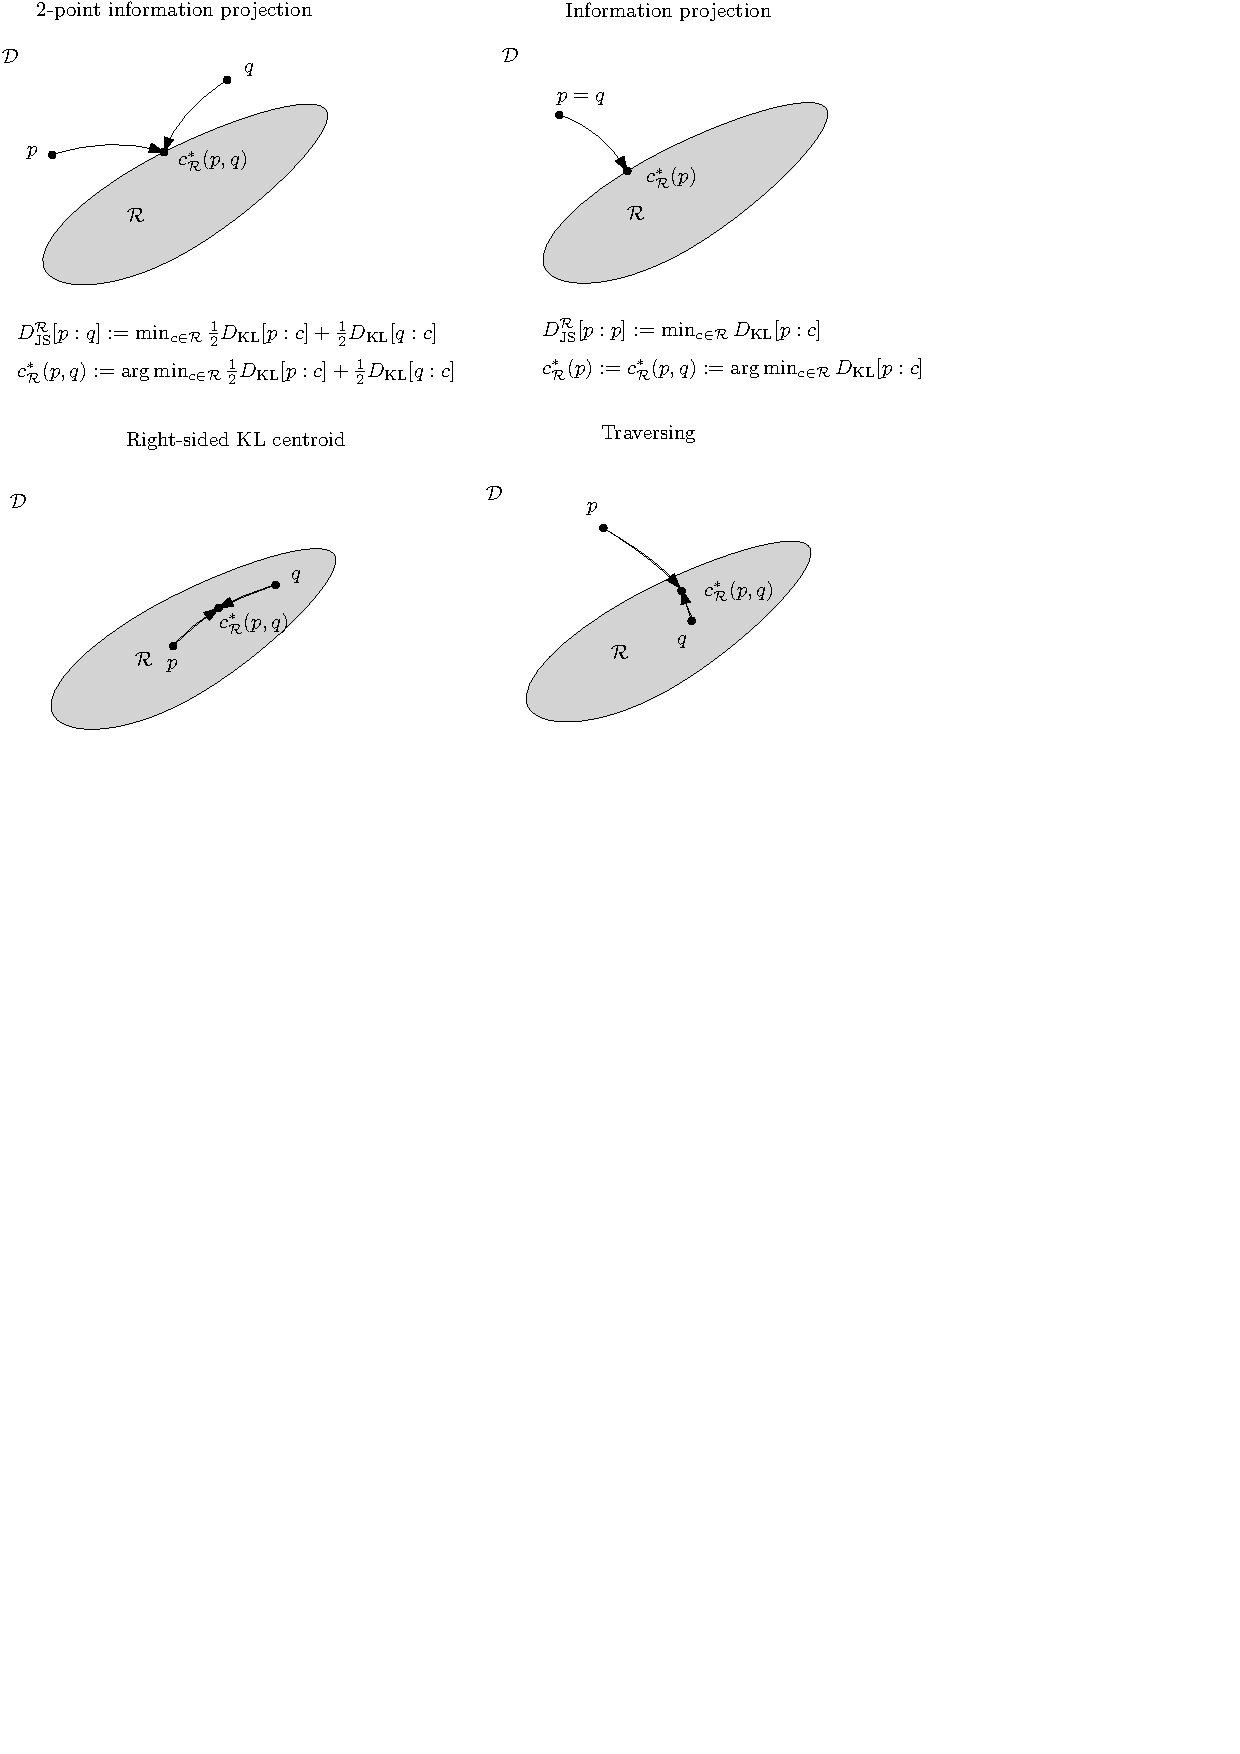
\includegraphics[width=0.9\textwidth]{FigIpe-relvJSdiv.pdf}

\caption{Illustrating several cases of the relative Jensen--Shannon divergence based on whether $p\in\calR$ and $q\in\calR$ or~not.\label{fig:relJS}}
\end{figure}
\begin{paracol}{2}
%\linenumbers
\switchcolumn

\vspace{-12pt}


%%%
\subsection{Relative Jensen--Shannon Divergences: Applications to Density Clustering and~Quantization}
\label{sec:relJSD}\label{sec:clustering}
%%%%

Let $D_\KL[p:q_\theta]$ be the Kullback--Leibler divergence between an {\em arbitrary} density $p$ and a density $q_\theta$ of an exponential family $\calQ=\{q_\theta\ :\ \theta\in\Theta\}$. 
Let us canonically express~\cite{EF-2009,EF-2014} the density $q_\theta(x)$, as~
$$
q_\theta(x)=\exp\left(\theta^\top t_\calQ(x)-F_\calQ(\theta)+k_\calQ(x)\right),
$$ 
where $t_\calQ(x)$ denotes the sufficient statistics, $k_\calQ(x)$ is an auxiliary carrier measure term (e.g., $k(x)=0$ for the Gaussian family 
and $k(x)=\log(x)$ for the Rayleigh family~\cite{EF-2009}),  and~
$F_\calQ(\theta)$ the cumulant function.
Assume that we   know in closed-form the following~quantities:
\begin{itemize}
\item $m_p:=E_p[t_\calQ(x)]=\int p(x)t_\calQ(x) \dmu(x)$ and 
\item the Shannon entropy $h[p]=-\int p(x)\log p(x) \dmu(x)$ of $p$.
\end{itemize}
Subsequently, we can express the KLD using a semi-closed-form formula.

\begin{Proposition}\label{eq:kldmef}
Let $q_\theta\in\calQ$ be a density of an exponential family 
and $p$ an arbitrary density with $m_p=E_p[t_\calQ(x)]$.
Subsequently, the~Kullback--Leibler divergence between $p$ and $q_\theta$ is expressed  as:
\begin{equation}\label{eq:scfef}
D_\KL[p:q_\theta] = F_\calQ(\theta)-m_p^\top\theta-E_p[k_\calQ(x)]-h[p],
\end{equation}
where $h[p:q_\theta]=F_\calQ(\theta)-m_p^\top\theta-E_p[k_\calQ(x)]$ is the cross-entropy between $p$ and $q_\theta$.
\end{Proposition}

\begin{proof}
The proof is straightforward since $\log q_\theta(x)=\theta^\top t_\calQ(x)-F_\calQ(\theta)+k_\calQ(x)$.
Therefore, we have:
\begin{eqnarray}
D_\KL[p:q_\theta] &=& h[p:q_\theta]-h[p],\\
&=&-\int_\calX p(x)\log q_\theta(x) \dmu(x) - h[p],\\
&=& F_\calQ(\theta)-m_p^\top\theta-E_p[k_\calQ(x)]-h[p]. 
\end{eqnarray}
\end{proof}

\begin{Example}
For example, when $q_\theta=q_{\mu,\Sigma}$ is the density of a multivariate Gaussian distribution $\mathcal{N}(\mu,\Sigma)$ (with $k_\calN(x)=0$), we have
\begin{equation}
D_\KL[p:q_{\mu,\Sigma}]=\frac{1}{2}\left(\log |2\pi\Sigma|+
(\mu-m)^\top \Sigma^{-1}(\mu-m) + \tr(\Sigma^{-1}S) \right)-h[p],
\end{equation}
where $m=\mu(p)=E_p[X]$ and  $S=\mathrm{Cov}(p):=E_p\left[XX^\top\right]-E_p[X]E_p[X]^\top$.  
\end{Example}

The formula of Proposition~\ref{eq:kldmef} is said in semi-closed-form, because~it relies on knowing both the entropy $h$ of $p$ and the  sufficient statistic moments $E_p[t_\calQ(x)]$. 
Yet, this semi-closed formula may prove to be useful in practice:
For example, we can answer the comparison~predicate\\
\centerline{``Is $D_\KL[p:q_{\theta_1}]\geq D_\KL[p:q_{\theta_2}]$ or not?''} \\
by checking whether
$F_\calQ(\theta_1)-F_\calQ(\theta_2)-m_p^\top(\theta_1-\theta_2)\geq 0$ or not (i.e., the~terms $-E_p[k_\calQ(x)]-h[p]$ in Equation~(\ref{eq:scfef}) cancel out).
Thus, we get a closed-form predicate, although~$D_\KL$ is only known in semi-closed-form.
This KLD comparison predicate shall be used later on when clustering densities with respect to centroids in~Section \ref{sec:clustering}. 

\begin{Remark}
Note that when $Y=f(X)$ for an invertible and differentiable transformation $f$ then we have $h[Y]=h[X]+E_X[\log |J_f(X)|]$ where $J_f$ denotes the Jacobian matrix.
For example, when $Y=f(X)=AX$, we have $h[Y]=h[X]+\log |A|$.
\end{Remark}

When $p$ belongs to an exponential family $\calP$  ($\calP$ may be different from $\calQ$) with cumulant function $F_\calP$, sufficient statistics $t_\calP(x)$, 
auxiliary carrier term $k_\calP(x)$, and~natural parameter $\theta$, 
  we have the entropy~\cite{crossentropyEF-2010} expressed, as~follows:
\begin{eqnarray}
h[p] &=& F_\calP(\theta)-\theta^\top\nabla F_\calP(\theta)-E_p[k_\calP(x)],\\
&=& -F^*_\calP(\eta)-E_p[k_\calP(x)],
\end{eqnarray}
where $F^*_\calP(\eta)=\theta^\top\nabla F(\theta)-F(\theta)$ is the Legendre transform of $F(\theta)$ and $\eta=\eta(\theta)=\nabla F(\theta)$ is called 
the moment parameter since we have $\eta(\theta)=E_p[t_\calP(x)]$~\cite{EF-2009,EF-2014}.

It follows the following proposition refining Proposition~\ref{eq:kldmef} when $p=p_\theta\in\calP$:

\begin{Proposition}\label{eq:klddiffef}
Let $p_{\theta}$ be a density of an exponential family $\calP$ and
 $q_{\theta'}$ be a density of an exponential family $\calQ$. 
Subsequently, the~Kullback--Leibler divergence between $p_{\theta}$ and $q_{\theta'}$ is expressed  as:
\begin{equation}\label{eq:htimesk}
D_\KL[p_{\theta}:q_{\theta'}] = 
F_\calQ(\theta')+F_\calP^*(\eta)-E_{p_{\theta}}[t_\calQ(x)]^\top\theta' +E_{p_{\theta}}[k_\calP(x)-k_\calQ(x)].
\end{equation}
\end{Proposition}


\begin{proof}
We have
\begin{eqnarray}
D_\KL[p_{\theta}:q_{\theta'}] &=& h[p_{\theta}:q_{\theta'}]-h[p_{\theta}],\\
&=&  F_\calQ(\theta')-m_{p_\theta}^\top\theta'-E_{p_{\theta}}[k_\calQ(x)] + F^*_\calP(\eta)+E_{p_{\theta}}[k_\calP(x)],\\
&=& F_\calQ(\theta') + F^*_\calP(\eta)- E_{p_{\theta}}[t_\calQ(x)]^\top \theta' +E_{p_{\theta}}[k_\calP(x)-k_\calQ(x)].
\end{eqnarray}
\end{proof}

 

In particular, when $p$ and $q$ belong both to the same exponential family (i.e., $\calP=\calQ$ with $k_\calP(x)=k_\calQ(x)$), we have $F(\theta):=F_\calP(\theta):=F_\calQ(\theta)$ and $
E_{p_{\theta}}[t_\calQ(x)]=\nabla F(\theta)=:\eta$, and~
$$
D_\KL[p_{\theta}:q_{\theta'}]=F(\theta')+F^*(\eta)-\theta'^\top\eta.
$$
This last equation is the Fenchel--Young divergence in Bregman manifolds~\cite{FenchelYoung-2020,BregmanManifold-2021} (called dually flat spaces in information geometry~\cite{IG-2016}).
Thus the divergence can be rewritten as equivalent dual Bregman divergences:
\begin{eqnarray}
D_\KL[p_{\theta}:q_{\theta'}] &=& F(\theta')+F^*(\eta)-\eta^\top\theta',\\
&=& B_F(\theta':\theta),\\
&=& B_{F^*}(\eta:\eta'),
\end{eqnarray}
where $\eta'=\nabla F(\theta')$.


Notice that $D_\KL[p_\theta:\calQ]:=\min_{\theta'\in\Theta'} D_\KL[p_\theta:q_{\theta'}]$ is unique 
and can be calculated as $\eta'=\nabla F_\calQ(\theta')=E_{p_\theta}[t_\calQ(x)]$.


Let us report two examples of calculations of the KLD between two densities of two exponential~families.

\begin{Example}
For the first exponential family, consider the  family of Laplacian distributions:
$$
\calP=\calL=\left\{p_\sigma(x):=\frac{1}{2\sigma}\exp\left(-\frac{|x|}{\sigma}\right)\ :\ \sigma>0\right\}.
$$
The canonical decomposition of the density yields
 $t_\calL(x)=|x|$, $\theta=-\frac{1}{\sigma}$, $k_{\calL}(x)=0$, and~$F_\calL(\theta)=\log\frac{2}{-\theta}$.  
(i.e., $F_\calL(\theta(\sigma))=\log{2\sigma}$).
It follows that $\eta(\theta)=F_\calL'(\theta)=-\frac{1}{\theta}$  ($\eta(\sigma)=\sigma=E[|x|]$), $\theta(\eta)=-\frac{1}{\eta}$,
and $F_\calL^*(\eta)=-1-\log(2\eta)$ and, therefore, $F_\calL^*(\eta(\sigma))=-1-\log(2\sigma)$.

For the second family, consider the exponential family of zero-centered Gaussian distributions:
$$
\calQ=\calN_0=\left\{q_{\sigma'}(x)=\frac{1}{\sqrt{2\pi(\sigma')^2}}\exp\left(-\frac{x^2}{2(\sigma')^2}\right)\right\}.
$$
We have $t_{\calN_0}(x)=x^2$, $k_{\calN_0}(x)=0$, $\theta'=-\frac{1}{2(\sigma')^2}$, and~
$F_{\calN_0}(\sigma')=\frac{1}{2}\log(2\pi(\sigma')^2)$.

Moreover, let us calculate $E_{p_\sigma}[t_{\calN_0}(x)]=E_{p_{\sigma}}[x^2]=2\sigma^2$.
Subsequently, we can calculate the Kullback--Leibler divergence between $p_{\sigma}\sim\calL(\sigma)$ and $q_{\sigma'}\sim\calN_0(\sigma')$, as~follows:
\begingroup\makeatletter\def\f@size{9}\check@mathfonts
\def\maketag@@@#1{\hbox{\m@th\normalsize\normalfont#1}}%
\begin{eqnarray}
D_\KL[p_{\sigma}:q_{\sigma'}] &=& 
F_\calQ(\theta'(\sigma'))+F_\calP^*(\eta(\sigma))-E_{p_{\sigma}}[t_\calQ(x)]^\top\theta'(\sigma') +E_{p_{\sigma}}[k_\calP(x)-k_\calQ(x)],\\
&=& \frac{1}{2}\log(2\pi(\sigma')^2) - 1-\log(2\sigma) -2\sigma^2 \left(-\frac{1}{2(\sigma')^2}\right),\\
&=&\log\left(\frac{\sigma'}{\sigma}\right) +\left(\frac{\sigma}{\sigma'}\right)^2+\frac{1}{2}\log\left(\frac{\pi}{2}\right)-1.
\end{eqnarray}
\endgroup
Notice that $D_\KL[p_{\sigma}:q_{\sigma'}]\geq 0$, but~never $0$ since the $\calP\cap\calQ=\emptyset$.

Let us now compute the reverse Kullback--Leibler divergence $D_\KL[q_{\sigma'}:p_{\sigma}]$. 
We first calculate $E_{q_{\sigma'}}[t_{\calL}(x)]=E_{q_{\sigma'}(\sigma')}[|x|]=\sqrt{\frac{2}{\pi}}\sigma'$.
Since $F_\calQ(\theta')=\frac{1}{2}\log(\frac{\pi}{-\theta'})$, we have $\eta'(\theta')=F_\calQ'(\theta')=-\frac{1}{2\theta'}$.
Thus $\eta'(\sigma')=(\sigma')^2$ and $F^*_\calQ(\eta')=-\frac{1}{2}-\frac{1}{2}\log(2\pi\eta)$.
Therefore, we get $F_\calQ^*(\eta'(\sigma'))=-h[q_{\sigma'}]=-\frac{1}{2}\log(2\pi e(\sigma')^2)$.

It follows that
\begingroup\makeatletter\def\f@size{9}\check@mathfonts
\def\maketag@@@#1{\hbox{\m@th\normalsize\normalfont#1}}%
\begin{eqnarray}
D_\KL[q_{\sigma'}:p_{\sigma}] &=& 
F_\calP(\theta(\sigma))+F_\calQ^*(\eta'(\sigma'))-E_{q_{\theta'}}[t_\calP(x)]^\top\theta(\sigma) +E_{q_{\theta'}}[k_\calP(x)-k_\calQ(x)],\\
&=& \log (2\sigma)-\frac{1}{2}\log(2\pi e(\sigma')^2)-\sqrt{\frac{2}{\pi}}\sigma'\times\left(-\frac{1}{\sigma}\right),\\
&=& \sqrt{\frac{2}{\pi}}\frac{\sigma'}{\sigma}+\log\left(\frac{\sigma}{\sigma'}\right)-\frac{1}{2}\log(\frac{\pi}{2}e).
\end{eqnarray}
\endgroup
Again, we have $D_\KL[q_{\sigma'}:p_{\sigma}]\geq 0$, but~never $0$, because~$\calP\cap\calQ=\emptyset$.
\end{Example}


\begin{Example}\label{ex:Weibull}
Let us use the formula of Equation~(\ref{eq:htimesk}) to  calculate the KLD between two Weibull distributions~\cite{KLDWeibull-2013}.
A Weibull distribution of shape $\kappa>0$ and  scale  $\sigma>0$ has a density defined on $\calX=[0,\infty)$, as~follows:
$$
p^\Wei_{\kappa,\sigma}(x) := \frac{\kappa}{\sigma} \left(\frac{x}{\sigma}\right)^{\kappa-1} 
\exp\left(-\left(\frac{x}{\sigma}\right)^\kappa\right).
$$

For a fixed shape $\kappa$, the~set of Weibull distributions $\calW_\kappa:=\{p^\Wei_{\kappa,\sigma}\ :\ \sigma>0\}$ form an exponential family with natural parameter $\theta=-\frac{1}{\sigma^\kappa}$, sufficient statistic $t_\kappa(x)=x^\kappa$, 
auxiliary carrier term $k_\kappa(x)=(\kappa-1)\log x+\log \kappa$, and~cumulant function $F_\kappa(\theta)=-\log(-\theta)$ (so that 
$F_\kappa(\theta(\sigma))=F_\kappa(\sigma)=\kappa\log\sigma$):

$$
p^\Wei_{\kappa,\sigma}(x):=\exp\left(-\frac{1}{\sigma^\kappa} x^k +\log\frac{1}{\sigma^\kappa}+k(x)\right).
$$

We recover the exponential family of exponential distributions of rate parameter $\lambda=\frac{1}{\sigma}$ when $\kappa=1$:
\begin{eqnarray*}
p^\Exp_\lambda(x)&=&p^\Wei_{1,\sigma}(x)=\frac{1}{\sigma}\exp\left(-\frac{x}{\sigma}\right),\\
&=& \lambda\exp\left(-\lambda x\right),
\end{eqnarray*}
 and the exponential family of Rayleigh distributions when $\kappa=2$ with scale parameter $\sigma_\Ray=\frac{\sigma}{\sqrt{2}}$:
\begin{eqnarray*}
p^\Ray_{\sigma_\Ray}(x)&=&p^\Wei_{2,\sigma}(x)=\frac{2x}{\sigma^2}\exp\left(-\frac{x^2}{\sigma^2}\right),\\
&=&\frac{x}{\sigma_\Ray^2}\exp\left(-\frac{x^2}{2\sigma_\Ray^2}\right).
\end{eqnarray*}

Now, assume that we are given the differential entropy of the Weibull distributions~\cite{diffentropy-2013} (pp.~155--156):
$$
h\left[p^\Wei_{\kappa_1,\sigma_1}\right]=\gamma\left(1-\frac{1}{\kappa_1}\right)+\log\frac{\sigma_1}{\kappa_1}+1,
$$
where $\gamma\approx 0.5772156649$ is the Euler--Mascheroni constant, and~the Weibull raw moments~\cite{diffentropy-2013} (p.~155):
$$
m=E_{p^\Wei_{\kappa_1,\sigma}}\left[x^{\kappa_2}\right] = \sigma_1^{\kappa_2} \Gamma\left(1+\frac{\kappa_2}{\kappa_1}\right),
$$
where $\Gamma(x)=\int_0^\infty t^{x-1} e^{-t} \mathrm{d}t$ is the gamma function (with $\Gamma(n)=(n-1)!$ for integers $n$).
Because $h[p^\Wei_{\kappa,\sigma}]=F_\kappa(\theta)-\theta^\top\nabla F_\kappa(\theta)-E_{p^\Wei_{\kappa,\sigma}}[k_\kappa(x)]
=-F^*_\kappa(\eta)-E_{p^\Wei_{\kappa,\sigma}}[k_\kappa(x)]$, we deduce that
$$
E_{p^\Wei_{\kappa,\sigma}}[k_\kappa(x)]=-F_\kappa^*(\eta)-h\left[p^\Wei_{\kappa,\sigma}\right],
$$
where $F^*_\kappa(\eta)$ is the Legendre transform of $F_\kappa(\theta)$ and $\eta(\theta)=\nabla F_\kappa(\theta)=-\frac{1}{\theta}=E[t(x)]=E[x^\kappa]$.
We have $\theta(\eta)=\nabla F^*_\kappa(\eta)=-\frac{1}{\eta}$ and $F^*_\kappa(\eta)=\eta^\top\nabla F^*_\kappa(\eta)-F_\kappa(\nabla F^*_\kappa(\eta))=-1-\log\eta$.
It follows that 
$$
E_{p^\Wei_{\kappa,\sigma}}[k_\kappa(x)]=1+\log\left(\sigma\Gamma\left(1+\frac{1}{\kappa}\right)\right)-\gamma\left(1-\frac{1}{\kappa}\right)-\log\frac{\sigma}{\kappa}+1.
$$
Therefore, we deduce that the logarithmic moment of $p^\Wei_{\kappa_1,\sigma}$ is:
$$
E_{p^\Wei_{\kappa_1,\sigma}}[\log x]=-\frac{\gamma}{\kappa_1}+\log\sigma_1.
$$
This coincides with the explicit definite integral calculation reported in~\cite{KLDWeibull-2013}.

Subsequently, we calculate the KLD between two Weibull distributions using Equation~(\ref{eq:htimesk}), as~follows:
\begingroup\makeatletter\def\f@size{8}\check@mathfonts
\def\maketag@@@#1{\hbox{\m@th\normalsize\normalfont#1}}%
\begin{eqnarray}
D_\KL\left[p^\Wei_{\kappa_1,\sigma_1}:p^\Wei_{\kappa_2,\sigma_2}\right] &=& 
F_{\kappa_2}(\theta') + F^*_{\kappa_1}(\eta)- E_{p_{\kappa_1,\sigma_1}}[x^{\kappa_2}]^\top \theta' +E_{p_{\kappa_1,\sigma_1}}[k_{\kappa_1}(x)-k_{\kappa_2}(x)]
\\
&=& \log \frac{\kappa_{1}}{\sigma_{1}^{\kappa_{1}}}-\log \frac{\kappa_{2}}{\sigma_{2}^{\kappa_{2}}}+
\left(\kappa_{1}-\kappa_{2}\right)\left[\log \sigma_{1}-\frac{\gamma}{\kappa_{1}}\right]+\left(\frac{\sigma_{1}}{\sigma_{2}}\right)^{\kappa_{2}} \Gamma\left(\frac{\kappa_{2}}{\kappa_{1}}+1\right)-1\\ \nonumber\vspace{-6pt}
\end{eqnarray}
\endgroup
since we have the following terms:
\begin{eqnarray*}
F_{\kappa_2}(\theta') &=&  \log \sigma_2^{\kappa_2},\\
F^*_{\kappa_1}(\eta) &=&  -1-\log \sigma_1^{\kappa_1},\\
- E_{p_{\kappa_1,\sigma_1}}[x^{\kappa_2}]^\top \theta' &=& \frac{1}{\sigma_2^{\kappa_2}} \sigma_1^{\kappa_2}\Gamma\left(1+\frac{\kappa_2}{\kappa_1}\right)\\
E_{p_{\kappa_1,\sigma_1}}[k_{\kappa_1}(x)-k_{\kappa_2}(x)] &=& (\kappa_1-\kappa_2)E_{p_{\kappa_1,\sigma_1}}[\log x]+\log\frac{\kappa_1}{\kappa_2},\\
&=& \log\frac{\kappa_1}{\kappa_2} +  (\kappa_1-\kappa_2)\left(\log\sigma_1-\frac{\gamma}{\kappa_1}\right).
\end{eqnarray*}

This formula matches the formula reported in~\cite{KLDWeibull-2013}.

When $\kappa_1=\kappa_2=1$, we recover the ordinary KLD formula between two exponential distributions~\cite{EF-2009} with $\lambda_i=\frac{1}{\sigma_i}$ since $\Gamma(2)=(2-1)!=1$:
\begin{eqnarray}
D_\KL\left[p^\Wei_{1,\sigma_1}:p^\Wei_{1,\sigma_2}\right] &=&  \log\frac{\sigma_2}{\sigma_1}+ \frac{\sigma_1}{\sigma_2}-1,\\
&=& \frac{\lambda_2}{\lambda_1}-\log\frac{\lambda_2}{\lambda_1}-1.\label{eq:klexp}
\end{eqnarray}

When $\kappa_1=\kappa_2=2$, we recover the ordinary KLD formula between two Rayleigh distributions~\cite{EF-2009}, with~
$\sigma_\Ray=\frac{\sigma}{\sqrt{2}}$:
\begin{eqnarray}
D_\KL\left[p^\Wei_{2,\sigma_1}:p^\Wei_{2,\sigma_2}\right] &=&  \log\left(\frac{\sigma_2^2}{\sigma_1^2}\right)+ \frac{\sigma_1^2}{\sigma_2^2}-1,\\
&=& \log\left(\frac{{\sigma_\Ray}_2^2}{{\sigma_\Ray}_1^2}\right)+ \frac{{\sigma_\Ray}_1^2}{{\sigma_\Ray}_2^2}-1.\label{eq:klray}
\end{eqnarray}

The formulae of Equations~(\ref{eq:klexp}) and~(\ref{eq:klray}) are linked by the fact that if $X\sim\mathrm{Exp}(\lambda)$ and $Y=\sqrt{X}$ then $Y\sim \mathrm{Ray}\left(\frac{1}{\sqrt{2\lambda}}\right)$, and~$f$-divergences~\cite{Csiszar-1967}, including the Kullback--Leibler divergence are invariant by a differentiable transformation~\cite{infoproj-2021}.
\end{Example}



Jeffreys' divergence symmetrizes the KLD divergence, as~follows:
\begin{equation}
D_J[p:q] := D_\KL[p:q]+D_\KL[q:p]=2A(D_\KL[p:q],D_\KL[q:p]).
\end{equation}
The Jeffreys divergence between two densities of different exponential families $\calP$ and $\calQ$ is
% start a new page without indent 4.6cm
%\clearpage
\end{paracol}
\nointerlineskip
\begin{equation}
D_J[p_\theta:q_{\theta'}]=\theta'^\top(\eta'-E_{p_\theta}[t_\calQ(x)])+\theta^\top(\eta-E_{q_{\theta'}}[t_\calP(x)])
+E_{p_\theta}[k_\calP(x)-k_\calQ(x)]+E_{q_{\theta'}}[k_\calQ(x)-k_\calP(x)].
\end{equation}
\begin{paracol}{2}
%\linenumbers
\switchcolumn

When $\calP=\calQ$, we have $E_{p_\theta}[t_\calQ(x)]=\eta$ and $E_{q_{\theta'}}[t_\calP(x)])=\eta'$, so that we find the usual expression
of the Jeffreys divergence between two densities of an exponential family:
\begin{equation}
D_J[p_\theta:p_{\theta'}]=(\theta'-\theta)^\top (\eta'-\eta).
\end{equation}



To find the best density $q_\theta$ approximating $p$ by minimizing $\min_{\theta} D_\KL[p:q_\theta]$, we solve $\nabla F(\theta)=\eta=m$ and, therefore,
$\theta=\nabla F^*(m)=(\nabla F)^{-1}(m)$, where $F^*(\eta)=E_{q_\eta}[\log q_\eta(m)]$, with~$F^*$ denoting the Legendre--Fenchel convex conjugate~\cite{EF-2014}.
In particular, when $p=\sum w_i p_{\theta_i}$ is a mixture of EFs (with $m=E_p[t(x)]=\sum w_i\eta_i$ with $\eta_i=E_{p_{\theta_i}}[t(x)]$ thanks to the linearity of the expectation), then the best density of the EF simplifying $p$ is
\begin{eqnarray}
\min_\theta D_\KL[p:q_\theta] &=& \min_\theta F(\theta)-m^\top\theta,\\
&=& \min_\theta F(\theta)-\sum w_i\eta_i^\top\theta.
\end{eqnarray}

Taking the gradient with respect to $\theta$, we have $\nabla F(\theta)=\eta=\sum w_i\eta_i$.
This yields another proof without the Pythagoras theorem~\cite{Pelletier-2005,LearningMixtureKde-2013}.

\begin{Proposition}\label{prop:mixsinglecomponent}
Let $m(x)=\sum w_i p_{\theta_i}(x)$ be a mixture with components that belong to an exponential family with cumulant function $F$.
Subsequently, $\theta^*=\arg_\theta \min_{\theta} D_\KL[p:q_\theta]$ is $\nabla F^*(\sum_{i=1}^n w_i\eta_i)$, where the $\eta_i=\nabla F(\theta_i)$ are the moment parameters of the mixture components.
\end{Proposition}


Consider the following two problems:

\begin{Problem}[Density clustering]\label{pb:dc}
Given a set of $n$ weighted densities $(w_1,p_1), \ldots, (w_n,p_n)$, partition them into $k$ clusters $\calC_1,\ldots,\calC_k$ in order to minimize the $k$-centroid objective function with respect to a statistical divergence $D$:
$\sum_{i=1}^n w_i \min_{l\in\{1,\ldots,k\}}  D[p_i:c_l]$, where $c_l$ denotes the centroid of cluster $\calC_l$ for $l\in\{1,\ldots,k\}$.
\end{Problem}

For example, when all the densities $p_i$'s are isotropic Gaussians, we recover the $k$-means objective function~\cite{kmeans-1982}.


\begin{Problem}[Mixture component quantization]\label{pb:mq}
Given a statistical mixture $m(x)=\sum_{i=1}^n w_i$ $p_i(x)$, quantize the mixture components into $k$ densities $q_1,\ldots, q_k$ in order to minimize
$\sum_i w_i $  $ \min_{l\in\{1,\ldots,k\}}D[p_i:q_l]$.
\end{Problem}

Notice that, in~Problem~\ref{pb:dc}, the~input densities $p_i$'s may be mixtures, i.e.,~$p_i(x)=\sum_{j=1}^{n_i} w_{i,j}p_{i,j}(x)$.
Using the relative information radius, we can cluster a set of distributions (potentially mixtures) into an exponential family mixture, or~quantize an exponential family mixture.
Indeed, we can implement an extension of $k$-means~\cite{kmeans-1982} with $k$-centers $q_{\theta_i}$, to~assign density $p_i$ to cluster $C_j$ (with center $q_j$), we need to perform basic comparison tests
$D_\KL[p_i:q_{\theta_l}]\geq D_\KL[p_i:q_{\theta_j}]$. 
Provided that the cumulant $F$ of the exponential family is in closed-form, we do not need formula for the entropies $h(p_i)$.

Clustering and quantization of densities/mixtures have been widely studied in the literature, see, for~example,~\cite{EntropicClusteringGaussians-2006,ClusteringGaussian-2008,QuantizationBregman-2010,SimplifyingMixtures-2010,ClusteringGMM-2013,MusicGMM-2015,ClusteringGaussian-2016}.




%%%
\section{Conclusions}\label{sec:concl}
%%%%



To summarize, the~ordinary Jensen--Shannon divergence has been defined in three equivalent ways in the literature:
\begin{eqnarray}
D_\JS[p,q] &:=& \min_{c\in\calD} \frac{1}{2}\left( D_\KL[p:c]+D_\KL[q:c] \right),\label{eq:js1}\\ 
&=&  \frac{1}{2}\left(D_\KL\left[p:\frac{p+q}{2}\right]+D_\KL\left[q:\frac{p+q}{2}\right]\right),\label{eq:js2}\\ 
&=&  h\left[\frac{p+q}{2}\right] - \frac{h[p]+h[q]}{2}. \label{eq:js3}
\end{eqnarray} 

The JSD Equation~(\ref{eq:js1}) was studied by Sibson in 1969 within the wider scope of information radius~\cite{Sibson-1969}:
Sibson relied on the R\'enyi $\alpha$-divergences (relative R\'enyi $\alpha$-entropies~\cite{Entropy-1995})
 and recovered the ordinary Jensen--Shannon divergence as a particular case of the $\alpha$-information radius when $\alpha=1$ and $n=2$ points. The~$\alpha$-information radii are related to generalized Bhattacharyya distances with respect to power means and the total variation distance in the limit case of $\alpha=\infty$.



Lin~\cite{JS-1991} investigated the JSD Equation~(\ref{eq:js2}) in 1991 with its connection to the JSD defined in Equation~(\ref{eq:js2})).
In Lin~\cite{JS-1991}, the~JSD is interpreted as the arithmetic symmetrization of the $K$-divergence~\cite{nielsen2010family}.
Generalizations of the JSD based on Equation~(\ref{eq:js2}) were proposed in~\cite{JSsym-2019} using a generic mean instead of the arithmetic mean.
One motivation was to obtain a closed-form formula for the geometric JSD between multivariate Gaussian distributions, which relies on the geometric mixture (see~\cite{VIGJSD-2020} for a use case of that formula in deep learning).
Indeed, the~ordinary JSD between Gaussians is not available in closed-form (not analytic).
However, the~JSD between Cauchy distributions admit a closed-form formula~\cite{CauchyJSD-2021}, despite the calculation of a definite integral of a log-sum term. Instead of using an abstract mean to define a mid-distribution of two densities, one may also consider the mid-point of a geodesic linking these two densities (the arithmetic means $\frac{p+q}{2}$ is interpreted as a geodesic midpoint). 
Recently, Li~\cite{TransportInfoBD-2021} investigated the transport Jensen--Shannon divergence as a symmetrization of the Kullback--Leibler divergence in the $L^2$-Wasserstein space. 
See Section~5.4 of~\cite{TransportInfoBD-2021} and the closed-form formula of Equation~(18) obtained for the transport Jensen--Shannon divergence between two multivariate Gaussian~distributions.

The generalization of the identity between the JSD of Equation~(\ref{eq:js2}) and the JSD of Equation~(\ref{eq:js3}) was studied while using a skewing vector in~\cite{JScentroid-2020}. 
Although the JSD is a $f$-divergence~\cite{Csiszar-1964,JScentroid-2020}, the~Sibson-$M$ Jensen--Shannon symmetrization of a distance does not belong, in~general, to~the class of $f$-divergences.
The variational JSD definition of \mbox{Equation~(\ref{eq:js1})} is implicit, while the definitions of Equations~(\ref{eq:js2}) and~(\ref{eq:js3}) are explicit because the unique optimal centroid $c^*=\frac{p+q}{2}$ has been plugged into the objective function that was minimized by Equation~(\ref{eq:js1}).


In this paper, we proposed a generalization of the Jensen--Shannon divergence based on the variational definition of the ordinary Jensen--Shannon divergence based on the variational JSD definition of Equation~(\ref{eq:js1}): $D_\vJS[p:q]=\min_c \frac{1}{2}(D_\KL[p:c]+D_\KL[q:c])$.
We introduced the Jensen--Shannon symmetrization of an arbitrary divergence $D$ by considering a generalization of the information radius with respect to an abstract weighted mean $M_\beta$: $D^\vJS_M[p:q]:=\min_c M_\beta(D[p:c],D[q:c])$.
Notice that, in~the variational JSD, the~mean $M_\beta$ is used for averaging divergence values, while the mean $M_\alpha$ in the $(M_\alpha,N_\beta)$ JSD is used to define generic statistical mixtures.
We also consider relative variational JS symmetrization when the centroid has to belong to a prescribed family of densities.
For the case of exponential family, we showed how to compute the relative centroid in closed form, thus extending the pioneering work of Sibson, who considered the relative normal centroid used to calculate the relative normal information radius. 
Figure~\ref{fig:genJSdiag} illustrates the three generalizations of the ordinary skewed Jensen--Shannon divergence.
Notice that, in~general, the~$(M,N)$-JSDs and the variational JDSs are not $f$-divergences (except in the ordinary case).


% start a new page without indent 4.6cm
\clearpage
\end{paracol}
\nointerlineskip
\begin{figure}[H]
\widefigure
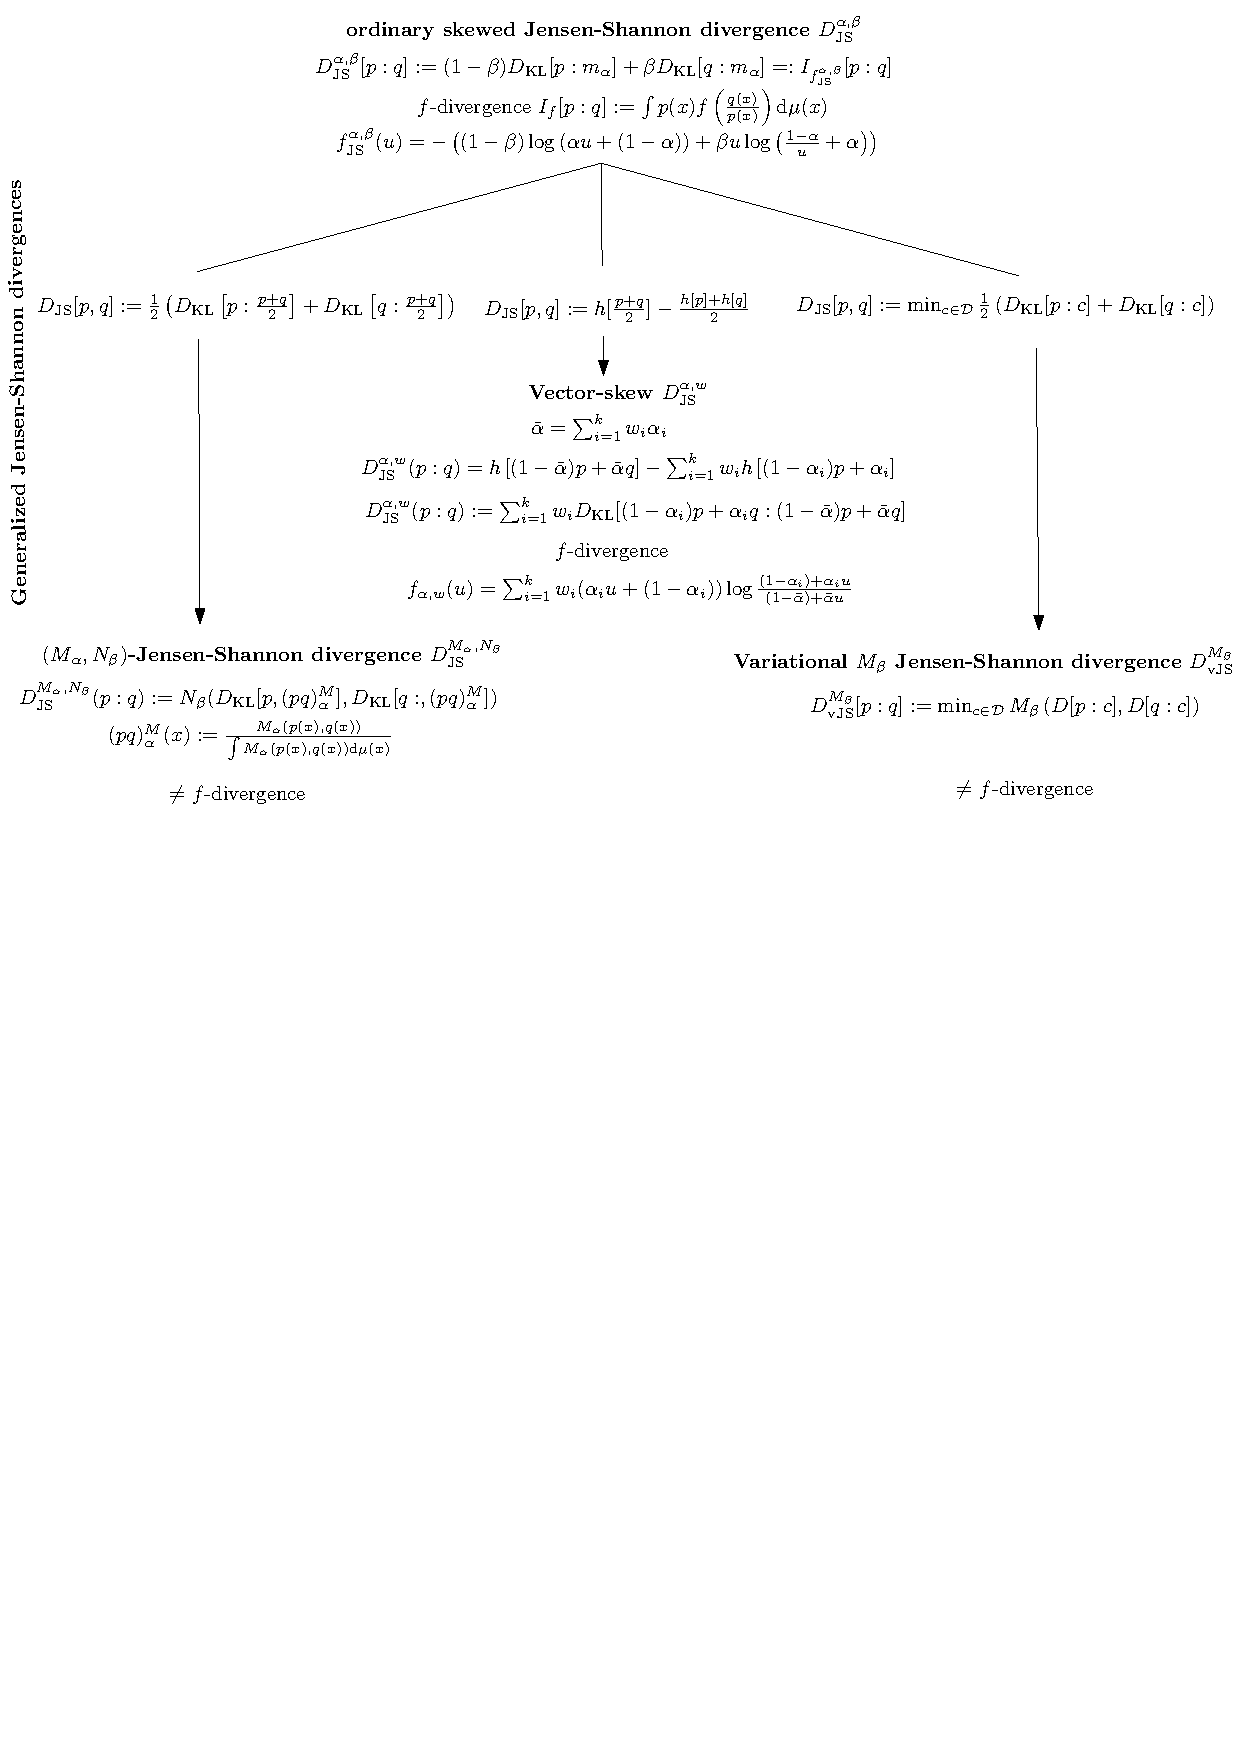
\includegraphics[width=0.9\textwidth]{FigIpe-GenJSDs.pdf}
\caption{{Three equivalent expressions}
 of the ordinary (skewed) Jensen-Shannon divergence which yield three different~generalizations.\label{fig:genJSdiag}}
\end{figure}
\begin{paracol}{2}
%\linenumbers
\switchcolumn

In a similar vein, Chen~et~al.~\cite{Chen-BD2-2008} considered the following minimax symmetrization of the scalar Bregman divergence~\cite{Bregman-1967}:
% start a new page without indent 4.6cm
%\clearpage
\end{paracol}
\nointerlineskip
\begin{eqnarray}\label{eq:varbd}
B^\minmax_f(p,q) &:=& \min_c \max_{\lambda\in[0,1]} \lambda B_f(p:c)+(1-\lambda) B_f(q:c),\\
&=& \max_{\lambda\in[0,1]} \lambda B_f(p:\lambda p+(1-\lambda) q)+(1-\lambda) B_f(q:\lambda p+(1-\lambda)),\\
&=& \lambda f(p)+(1-\lambda)f(q)-f(\lambda p+(1-\lambda))
\end{eqnarray}
\begin{paracol}{2}
%\linenumbers
\switchcolumn

\noindent where $B_f$ denotes the scalar Bregman divergence induced by a strictly convex and smooth function $f$:
\begin{equation}
B_f(p:q)=f(p)-f(q)-(p-q)f'(q).
\end{equation}
They proved that $\sqrt{B^\minmax_f(p,q)}$ yields a metric when $3(\log f'')''\geq ((\log f'')')^2$, and~extend the definition to the vector case and conjecture that the square-root metrization still holds in the multivariate case. 
In a sense, this definition geometrically highlights the notion of radius, since the minmax optimization amount to find a smallest enclosing ball enclosing~\cite{minmax-2013} the source distributions. The~circumcenter, also called the Chebyshev center~\cite{ChebyshevAlphaDiv-2020}, is then the mid-distribution instead of the centroid for the information radius.
The term "information radius'' is well-suited to measure the distance between two points for an arbitrary distance $D$.
Indeed, the~JS-symmetrization of $D$
 is defined by  $D^\JS[p:q]:=\min_c \{\frac{1}{2}D[p:c]+\frac{1}{2}D[q:c]\}$.
When $D[p:q]=D_E[p:q]=\|p-q\|$ is the Euclidean distance, we have $c=\frac{p+q}{2}$, and~
$D[p:c]=D[q:c]=\frac{1}{2}\|p-q\|=:r$ (i.e., the~radius being half of the diameter $\|p-q\|$). 
Thus, $D^\JS_E[p:q]=r$; hence, the~term chosen by Sibson~\cite{Sibson-1969} for $D^\JS$: information radius.
Besides providing another viewpoint, variational definitions of divergences have proven to be useful in practice (e.g., for~estimation).
For example, a~variational definition of the R\'enyi divergence generalizing the Donsker--Varadhan variational formula of the KLD is given in~\cite{variationalRenyi-2020}, which is used to estimate the R{\'e}nyi Divergences.  


\vspace{6pt} 

%\authorcontributions{}%For research articles with several authors, a~short paragraph specifying their individual contributions must be provided. The~following statements should be used ``Conceptualization, X.X. and Y.Y.; methodology, X.X.; software, X.X.; validation, X.X., Y.Y. and Z.Z.; formal analysis, X.X.; investigation, X.X.; resources, X.X.; data curation, X.X.; writing---original draft preparation, X.X.; writing---review and editing, X.X.; visualization, X.X.; supervision, X.X.; project administration, X.X.; funding acquisition, Y.Y. All authors have read and agreed to the published version of the manuscript.'', please turn to the  \href{http://img.mdpi.org/data/contributor-role-instruction.pdf}{CRediT taxonomy} for the term explanation. Authorship must be limited to those who have contributed substantially to the work~reported.

\funding{This research received no external funding}%Please add: ``This research received no external funding'' or ``This research was funded by NAME OF FUNDER grant number XXX.'' and  and ``The APC was funded by XXX''. Check carefully that the details given are accurate and use the standard spelling of funding agency names at \url{https://search.crossref.org/funding}, any errors may affect your future~funding.

%\institutionalreview{}%In this section, please add the Institutional Review Board Statement and approval number for studies involving humans or animals. Please note that the Editorial Office might ask you for further information. Please add “The study was conducted according to the guidelines of the Declaration of Helsinki, and~approved by the Institutional Review Board (or Ethics Committee) of NAME OF INSTITUTE (protocol code XXX and date of approval).” OR “Ethical review and approval were waived for this study, due to REASON (please provide a detailed justification).” OR “Not applicable” for studies not involving humans or animals. You might also choose to ex-clude this statement if the study did not involve humans or~animals.

\informedconsent{Not applicable}%Any research article describing a study involving humans should contain this statement. Please add “Informed consent was obtained from all subjects involved in the study.” OR “Patient con-sent was waived due to REASON (please provide a detailed justification).” OR “Not applicable” for studies not involving humans. You might also choose to exclude this statement if the study did not involve humans. Written informed consent for publication must be obtained from participating patients who can be identified (including by the patients themselves). Please state “Written informed consent has been obtained from the patient(s) to publish this paper” if~applicable.

%\dataavailability{} %In this section, please provide details regarding where data supporting reported results can be found, including links to publicly archived datasets analyzed or generated during the study. Please refer to suggested Data Availability Statements in section “MDPI Research Data Policies” at \href{https://www.mdpi.com/ethics}{https://www.mdpi.com/ethics}. You might choose to exclude this statement if the study did not report any~data.

%\vskip 0.5cm
%\noindent{\bf Acknowledgments}: 

\acknowledgments{We warmly thank Rob Brekelmans (Information Sciences Institute, University of Southern California, USA) for discussions and feedback related to the contents of this work. The~author thanks the reviewers for valuable feedback, comments, and~suggestions, and Ga\"etan Hadjeres (Sony CSL Paris) for his careful reading of the manuscript.}

\conflictsofinterest{The authors declare no conflict of interest.}% Declare conflicts of interest or state ``The authors declare no conflict of interest.'' Authors must identify and declare any personal circumstances or interest that may be perceived as inappropriately influencing the representation or interpretation of reported research results. Any role of the funders in the design of the study; in the collection, analyses or interpretation of data; in the writing of the manuscript, or~in the decision to publish the results must be declared in this section. If~there is no role, please state ``The funders had no role in the design of the study; in the collection, analyses, or~interpretation of data; in the writing of the manuscript, or~in the decision to publish the~results''.

\end{paracol}
\reftitle{References}
\begin{thebibliography}{999}
\providecommand{\natexlab}[1]{#1}

\bibitem[Sibson(1969)]{Sibson-1969}
Sibson, R.
\newblock Information radius.
\newblock {\em Z.  Wahrscheinlichkeitstheorie   Verwandte Geb.} {\bf 1969}, {\em 14},~149--160.

\bibitem[Barndorff-Nielsen(2014)]{EF-2014}
Barndorff-Nielsen, O.
\newblock {\em Information and Exponential Families: In Statistical Theory};
  John Wiley \& Sons:  {Hoboken, NJ, USA,}  
  2014.

\bibitem[Billingsley(2008)]{Billingsley-2008}
Billingsley, P.
\newblock {\em Probability and Measure}; John Wiley \& Sons:  {Hoboken, NJ, USA,}  2008.


\bibitem[Kullback(1997)]{Kullback-1997}
Kullback, S.
\newblock {\em Information Theory and Statistics}; Courier Corporation: {Chelmsford, MA, USA},  1997.

\bibitem[Cover and Thomas(2012)]{CoverThomasIT-2012}
Cover, T.M.; Thomas, J.A.
\newblock {\em Elements of Information Theory}; John Wiley \& Sons:  {Hoboken, NJ, USA,}  2012.


\bibitem[Lin(1991)]{JS-1991}
Lin, J.
\newblock {Divergence measures based on the Shannon entropy}.
\newblock {\em IEEE Trans. Inf. Theory} {\bf 1991}, {\em
  37},~145--151.

\bibitem[Morimoto(1963)]{fdivMorimoto-1963}
Morimoto, T.
\newblock {Markov processes and the $H$-theorem}.
\newblock {\em J. Phys. Soc. Jpn.} {\bf 1963}, {\em
  18},~328--331.

\bibitem[Csisz{\'a}r(1964)]{Csiszar-1964}
Csisz{\'a}r, I.
\newblock Eine informationstheoretische ungleichung und ihre anwendung auf
  beweis der ergodizitaet von markoffschen ketten.
\newblock {\em Magyer Tud. Akad. Mat. Kut. Int. Koezl.} {\bf 1964}, {\em
  8},~85--108.

\bibitem[Ali and Silvey(1966)]{fdiv-AliSilvey-1966}
Ali, S.M.; Silvey, S.D.
\newblock A general class of coefficients of divergence of one distribution
  from another.
\newblock {\em J. R. Stat. Soc. Ser. B (Methodological)} {\bf 1966}, {\em 28},~131--142.

\bibitem[Amari(2016)]{IG-2016}
Amari, S.i.
\newblock {\em Information Geometry and Its Applications}; Applied Mathematical
  Sciences; Springer: Tokyo, Japan,  2016.

\bibitem[McLachlan and Peel(2004)]{Mixtures-2004}
McLachlan, G.J.; Peel, D.
\newblock {\em Finite Mixture Models}; John Wiley \& Sons: {Hoboken, NJ, USA,}  2004.

\bibitem[Nielsen and Boltz(2011)]{BR-2011}
Nielsen, F.; Boltz, S.
\newblock {The Burbea-Rao and Bhattacharyya centroids}.
\newblock {\em IEEE Trans. Inf. Theory} {\bf 2011}, {\em
  57},~5455--5466.

\bibitem[Endres and Schindelin(2003)]{JSmetric-2003}
Endres, D.M.; Schindelin, J.E.
\newblock A new metric for probability distributions.
\newblock {\em IEEE Trans. Inf. Theory} {\bf 2003}, {\em
  49},~1858--1860.

\bibitem[Fuglede and Topsoe(2004)]{JSmetric-2004}
Fuglede, B.; Topsoe, F.
\newblock {Jensen-Shannon divergence and Hilbert space embedding}.
\newblock   In Proceedings of the International Symposium onInformation Theory, 2004. ISIT 2004.  Proceedings, {Chicago, IL, USA, 27 June--2 July} 2004;  IEEE: {Piscataway, NJ, USA,}  2004; p.~31.

\bibitem[Virosztek(2021)]{QuantumJSD-2021}
Virosztek, D.
\newblock {The metric property of the quantum Jensen-Shannon divergence}.
\newblock {\em Adv. Math.} {\bf 2021}, {\em 380},~107595,
\newblock
  doi:{\changeurlcolor{black}\href{https://doi.org/https://doi.org/10.1016/j.aim.2021.107595}{\detokenize{10.1016/j.aim.2021.107595}}}.

\bibitem[Goodfellow \em{et~al.}(2014)Goodfellow, Pouget-Abadie, Mirza, Xu,
  Warde-Farley, Ozair, Courville, and Bengio]{GAN-2014}
Goodfellow, I.J.; Pouget-Abadie, J.; Mirza, M.; Xu, B.; Warde-Farley, D.;
  Ozair, S.; Courville, A.; Bengio, Y.
\newblock Generative adversarial networks.
\newblock {\em arXiv Prepr.} {\bf 2014}, arXiv:1406.2661.

\bibitem[Goodfellow \em{et~al.}(2016)Goodfellow, Bengio, Courville, and
  Bengio]{DL-2016}
Goodfellow, I.; Bengio, Y.; Courville, A.; Bengio, Y.
\newblock {\em Deep Learning}; MIT Press: Cambridge, MA, USA, 2016.

\bibitem[Nielsen(2020)]{JScentroid-2020}
Nielsen, F.
\newblock {On a generalization of the Jensen--Shannon divergence and the
  Jensen--Shannon centroid}.
\newblock {\em Entropy} {\bf 2020}, {\em 22},~221.

\bibitem[Csisz{\'a}r(1967)]{EN-PhD-Csiszar-1967}
Csisz{\'a}r, I.
\newblock Information-type measures of difference of probability distributions
  and indirect observation.
\newblock {\em Stud. Sci. Math. Hung.} {\bf 1967}, {\em
  2},~229--318.

\bibitem[Csisz{\'a}r(2008)]{Csiszar-2008}
Csisz{\'a}r, I.
\newblock Axiomatic characterizations of information measures.
\newblock {\em Entropy} {\bf 2008}, {\em 10},~261--273.

\bibitem[Antol{\'\i}n \em{et~al.}(2009)Antol{\'\i}n, Angulo, and
  L{\'o}pez-Rosa]{JSApp-2009}
Antol{\'\i}n, J.; Angulo, J.; L{\'o}pez-Rosa, S.
\newblock {Fisher and Jensen--Shannon divergences: Quantitative comparisons
  among distributions. application to position and momentum atomic densities}.
\newblock {\em  J. Chem. Phys.} {\bf 2009}, {\em 130},~074110.

\bibitem[Nielsen(2019)]{JSsym-2019}
Nielsen, F.
\newblock {On the Jensen--Shannon symmetrization of distances relying on
  abstract means}.
\newblock {\em Entropy} {\bf 2019}, {\em 21},~485.

\bibitem[Nielsen(2010)]{nielsen2010family}
Nielsen, F.
\newblock {A family of statistical symmetric divergences based on Jensen's
  inequality}.
\newblock {\em arXiv Prepr.} {\bf 2010}, arXiv:1009.4004.

\bibitem[Nielsen and Nock(2017)]{JensenComparative-2017}
Nielsen, F.; Nock, R.
\newblock {Generalizing skew Jensen divergences and Bregman divergences with
  comparative convexity}.
\newblock {\em IEEE Signal Process. Lett.} {\bf 2017}, {\em
  24},~1123--1127.

\bibitem[de~Carvalho(2016)]{de2016mean}
de~Carvalho, M.
\newblock Mean, what do you Mean?
\newblock {\em  Am. Stat.} {\bf 2016}, {\em 70},~270--274.

\bibitem[Bullen(2013)]{Bullen-2013}
Bullen, P.S.
\newblock {\em Handbook of Means and Their Inequalities}; Springer
  Science \& Business Media: {Berlin/Heidelberg, Germany},  2013; Volume 560.

\bibitem[Niculescu and Persson(2018)]{WeightedMean-2018}
Niculescu, C.P.; Persson, L.E.
\newblock {\em {Convex Functions and Their Applications: A Contemporary
  Approach}}; Springer:  {Berlin/Heidelberg, Germany,}  
  2018.

\bibitem[Nielsen(2014)]{GenBhat-2014}
Nielsen, F.
\newblock {Generalized Bhattacharyya and Chernoff upper bounds on Bayes error
  using quasi-arithmetic means}.
\newblock {\em Pattern Recognit. Lett.} {\bf 2014}, {\em 42},~25--34.

\bibitem[Deasy \em{et~al.}(2020)Deasy, Simidjievski, and Li{\`o}]{VIGJSD-2020}
Deasy, J.; Simidjievski, N.; Li{\`o}, P.
\newblock {Constraining Variational Inference with Geometric Jensen-Shannon
  Divergence}.
\newblock   In Proceedings of the  {34th Conference on Neural Information Processing Systems (NeurIPS 2020), Vancouver, BC, Canada, 6--12 December} 2020.

\bibitem[Amari(2007)]{Amari-2007}
Amari, S.I.
\newblock Integration of stochastic models by minimizing $\alpha$-divergence.
\newblock {\em Neural Comput.} {\bf 2007}, {\em 19},~2780--2796.

\bibitem[Calin and Udriste(2014)]{IG-2014}
Calin, O.; Udriste, C.
\newblock {\em Geometric Modeling in Probability and Statistics}; Mathematics
  and Statistics;  Springer International Publishing:  {Berlin/Heidelberg, Germany,}  2014.

\bibitem[R{\'e}nyi \em{et~al.}(1961)R{\'e}nyi et~al.]{Renyi-1961}
R{\'e}nyi, A. 
\newblock On measures of entropy and information.
\newblock  In \emph{Proceedings of the Fourth Berkeley Symposium on Mathematical
  Statistics and Probability, Volume 1: Contributions to the Theory of
  Statistics}; The Regents of the University of California: {Oakland, CA, USA},  1961.

\bibitem[Blondel \em{et~al.}(2020)Blondel, Martins, and
  Niculae]{FenchelYoung-2020}
Blondel, M.; Martins, A.F.; Niculae, V.
\newblock {Learning with Fenchel-Young losses}.
\newblock {\em J. Mach. Learn. Res.} {\bf 2020}, {\em
  21},~1--69.

\bibitem[Faddeev(1957)]{Fadeev-1957}
Faddeev, D.K.
\newblock {Zum Begriff der Entropie einer endlichen
  Wahrscheinlichkeitsschemas}.
\newblock {\em Arbeiten zur Informationstheorie I}; Deutscher Verlag der
  Wissenschaften: {Berlin, Germany}, {1957}; pp. 85--90.

% Kolmogorov, A. (1930), “Sur la Notion de la Moyenne,” Atti della Academia Nazionale dei Lincei, 12, 323–343
\bibitem[Kolmogorov and Castelnuovo(1930)]{Kolmogorov-1930}
{Kolmogorov, A.N.; Castelnuovo, G.} 
\newblock {Sur la notion de la moyenne}. G. Bardi, Atti della Academia Nazionale dei Lincei,  Volume~12, pp. 323-–343, 1930.

\bibitem[Nagumo(1930)]{Nagumo-1930}
Nagumo, M.
\newblock {\"U}ber eine klasse der mittelwerte.
\newblock  \emph{Japanese Journal of Mathematics: Transactions and Abstracts}; The
  Mathematical Society of Japan: {Tokyo, Japan},  1930; Volume~7, pp. 71--79.

\bibitem[De~Finetti(1931)]{Finetti-1931}
De~Finetti, B.
\newblock {\em Sul Concetto di Media}; Istituto Italiano Degli Attuari:  {Roma, Italy},  1931.

\bibitem[Van~Erven and Harremos(2014)]{RenyiDiv-2014}
Van~Erven, T.; Harremos, P.
\newblock {R{\'e}nyi divergence and Kullback-Leibler divergence}.
\newblock {\em IEEE Trans. Inf. Theory} {\bf 2014}, {\em
  60},~3797--3820.

%  In Interpreting Multivariate Data, Barnett V. (ed.). Wiley: New York, 1981; 21–36.
\bibitem[Sibson(1981)]{Sibson-1981}
Sibson, R.
\newblock A brief description of natural neighbour interpolation.
\newblock {\em Interpret. Multivar. Data}; Barnett V. (ed.),
  John Wiley \& Sons:  {Hoboken, NJ, USA,}     {\bf 1981}, 21--36.
.

\bibitem[Boyd \em{et~al.}(2004)Boyd, Boyd, and Vandenberghe]{ConvexOptim-2004}
Boyd, S.; Boyd, S.P.; Vandenberghe, L.
\newblock {\em Convex Optimization}; Cambridge University Press: {Cambridge, UK},  2004.

\bibitem[Nielsen and Sun(2016)]{KLLSE-2016}
Nielsen, F.; Sun, K.
\newblock Guaranteed bounds on information-theoretic measures of univariate
  mixtures using piecewise log-sum-exp inequalities.
\newblock {\em Entropy} {\bf 2016}, {\em 18},~442.

\bibitem[Nielsen(2011)]{Chernoff-2011}
Nielsen, F.
\newblock Chernoff information of exponential families.
\newblock {\em arXiv Prepr.} {\bf 2011}, arXiv:1102.2684.

\bibitem[Nielsen(2013)]{Chernoff-2013}
Nielsen, F.
\newblock {An information-geometric characterization of Chernoff information}.
\newblock {\em IEEE Signal Process. Lett.} {\bf 2013}, {\em 20},~269--272.

\bibitem[Nielsen and Yvinec(1998)]{Nielsen-1998}
Nielsen, F.; Yvinec, M.
\newblock An output-sensitive convex hull algorithm for planar objects.
\newblock {\em Int. J. Comput. Geom. Appl.}
  {\bf 1998}, {\em 8},~39--65.

\bibitem[Nielsen and Nock(2013)]{fdivchiorder-2013}
Nielsen, F.; Nock, R.
\newblock On the chi square and higher-order chi distances for approximating
  $f$-divergences.
\newblock {\em IEEE Signal Process. Lett.} {\bf 2013}, {\em 21},~10--13.

\bibitem[Nielsen(2019)]{MinkowskiDiv-2019}
Nielsen, F.
\newblock {The statistical Minkowski distances: Closed-form formula for
  Gaussian mixture models}.
\newblock In \emph{International Conference on Geometric Science of Information};
  Springer:  {Berlin/Heidelberg, Germany,} 
  2019; pp. 359--367.

\bibitem[Fr{\'e}chet(1948)]{Frechet-1948}
Fr{\'e}chet, M.
\newblock Les {\'e}l{\'e}ments al{\'e}atoires de nature quelconque dans un
  espace distanci{\'e}.
\newblock {\em Ann.   L'Institut Henri Poincar{\'e}} {\bf 1948}, {\em
  10},~215--310.

\bibitem[Banerjee \em{et~al.}(2005)Banerjee, Merugu, Dhillon, and
  Ghosh]{BregmanKmeans-2005}
Banerjee, A.; Merugu, S.; Dhillon, I.S.; Ghosh, J.
\newblock Clustering with {B}regman divergences.
\newblock {\em J. Mach. Learn. Res.} {\bf 2005}, {\em
  6},~1705--1749.

\bibitem[Nielsen and Nock(2009)]{SBD-2009}
Nielsen, F.; Nock, R.
\newblock {Sided and symmetrized Bregman centroids}.
\newblock {\em IEEE Trans. Inf. Theory} {\bf 2009}, {\em
  55},~2882--2904.

\bibitem[Naudts(2011)]{Naudts-2011}
Naudts, J.
\newblock {\em Generalised Thermostatistics}; Springer Science \& Business
  Media:  {Berlin/Heidelberg, Germany,} 2011.

\bibitem[Tsallis(1988)]{Tsallis-1988}
Tsallis, C.
\newblock {Possible generalization of Boltzmann-Gibbs statistics}.
\newblock {\em J. Stat. Phys.} {\bf 1988}, {\em 52},~479--487.

\bibitem[Nielsen(2020)]{VoronoiCauchy-2020}
Nielsen, F.
\newblock {On Voronoi diagrams on the information-geometric Cauchy manifolds}.
\newblock {\em Entropy} {\bf 2020}, {\em 22},~713.

\bibitem[Nock \em{et~al.}(2015)Nock, Nielsen, and Amari]{conformaldiv-2015}
Nock, R.; Nielsen, F.; Amari, S.i.
\newblock On conformal divergences and their population minimizers.
\newblock {\em IEEE Trans. Inf. Theory} {\bf 2015}, {\em
  62},~527--538.

\bibitem[Brekelmans \em{et~al.}(2020{\natexlab{a}})Brekelmans, Nielsen,
  Makhzani, Galstyan, and Steeg]{LikelihoodRatioEF-2020}
Brekelmans, R.; Nielsen, F.; Makhzani, A.; Galstyan, A.; Steeg, G.V.
\newblock Likelihood Ratio Exponential Families.
\newblock {\em arXiv Prepr.} {\bf 2020}, arXiv:2012.15480.

\bibitem[Brekelmans \em{et~al.}(2020{\natexlab{b}})Brekelmans, Masrani, Bui,
  Wood, Galstyan, Steeg, and Nielsen]{AISqpath-2020}
Brekelmans, R.; Masrani, V.; Bui, T.; Wood, F.; Galstyan, A.; Steeg, G.V.;
  Nielsen, F.
\newblock Annealed Importance Sampling with $q$-Paths.
\newblock {\em arXiv Prepr.} {\bf 2020}, arXiv:2012.07823.

\bibitem[Nielsen(2020)]{nielsen2020generalization}
Nielsen, F.
\newblock A generalization of the $\alpha$-divergences based on comparable and
  distinct weighted means.
\newblock {\em arXiv Prepr.} {\bf 2020},  arXiv:2001.09660.

\bibitem[Amari and Ohara(2011)]{AmariOhara-2011}
Amari, S.i.; Ohara, A.
\newblock Geometry of $q$-exponential family of probability distributions.
\newblock {\em Entropy} {\bf 2011}, {\em 13},~1170--1185.

\bibitem[Grosse \em{et~al.}(2013)Grosse, Maddison, and
  Salakhutdinov]{Grosse-2013}
Grosse, R.; Maddison, C.J.; Salakhutdinov, R.
\newblock Annealing between distributions by averaging moments.
\newblock  In Proceedings of the 26th International Conference on Neural
  Information Processing Systems,   {Lake Tahoe, NV, USA, 5--8  December} 2013; pp. 2769--2777.

\bibitem[Nielsen(2018)]{InfProj-2018}
Nielsen, F.
\newblock What is an information projection?
\newblock {\em Not. AMS} {\bf 2018}, {\em 65},~321--324.

\bibitem[Nielsen and Garcia(2009)]{EF-2009}
Nielsen, F.; Garcia, V.
\newblock Statistical exponential families: A digest with flash cards.
\newblock {\em arXiv} {\bf 2009}, arXiv:0911.4863.

\bibitem[Nielsen and Nock(2010)]{crossentropyEF-2010}
Nielsen, F.; Nock, R.
\newblock Entropies and cross-entropies of exponential families.
\newblock  In Proceedings of the 2010 IEEE International Conference on Image Processing, {Hong Kong, China, 26--29 September} 2010; 
IEEE: {Piscataway, NJ, USA},  2010;
  pp. 3621--3624.

\bibitem[Nielsen(2021)]{BregmanManifold-2021}
Nielsen, F.
\newblock On Geodesic Triangles with Right Angles in a Dually Flat Space.
\newblock In {\em Progress in Information Geometry: Theory and Applications}; {Springer:  Berlin/Heidelberg, Germany,} 
 {2021}; pp. 153--190.

\bibitem[Bauckhage(2013)]{KLDWeibull-2013}
Bauckhage, C.
\newblock {Computing the Kullback-Leibler divergence between two Weibull
  distributions}.
\newblock {\em arXiv} {\bf 2013}, arXiv:1310.3713.

\bibitem[Michalowicz \em{et~al.}(2013)Michalowicz, Nichols, and
  Bucholtz]{diffentropy-2013}
Michalowicz, J.V.; Nichols, J.M.; Bucholtz, F.
\newblock {\em Handbook of Differential Entropy}; CRC Press:  {Boca Raton, FL, USA,}
  2013.

\bibitem[Csisz{\'a}r(1967)]{Csiszar-1967}
Csisz{\'a}r, I.
\newblock On topological properties of $f$-divergences.
\newblock {\em Stud. Math. Hungar.} {\bf 1967}, {\em 2},~329--339.

\bibitem[Nielsen(2021)]{infoproj-2021}
Nielsen, F.
\newblock On information projections between multivariate elliptical and
  location-scale families.
\newblock {\em arXiv Prepr.} {\bf 2021}, arXiv:2101.03839.

\bibitem[Pelletier(2005)]{Pelletier-2005}
Pelletier, B.
\newblock Informative barycentres in statistics.
\newblock {\em Ann. Inst. Stat. Math.} {\bf 2005},
  {\em 57},~767--780.

\bibitem[Schwander and Nielsen(2013)]{LearningMixtureKde-2013}
Schwander, O.; Nielsen, F.
\newblock Learning mixtures by simplifying kernel density estimators. In {\em
  Matrix Information Geometry}; Springer:  {Berlin/Heidelberg, Germany},  2013; pp. 403--426.

\bibitem[Lloyd(1982)]{kmeans-1982}
Lloyd, S.
\newblock {Least squares quantization in PCM}.
\newblock {\em IEEE Trans. Inf. Theory} {\bf 1982}, {\em
  28},~129--137.

\bibitem[Davis and Dhillon(2006)]{EntropicClusteringGaussians-2006}
Davis, J.V.; Dhillon, I.
\newblock {Differential entropic clustering of multivariate Gaussians}.
\newblock  In Proceedings of the 19th International Conference on Neural
  Information Processing Systems, {Vancouver, BC, Canada, 4--7 December} 2006; pp. 337--344.

\bibitem[Nielsen and Nock(2008)]{ClusteringGaussian-2008}
Nielsen, F.; Nock, R.
\newblock Clustering multivariate normal distributions.
\newblock  In \emph{Emerging Trends in Visual Computing}; Springer:  {Berlin/Heidelberg, Germany,}  2008; pp. 164--174.

\bibitem[Fischer(2010)]{QuantizationBregman-2010}
Fischer, A.
\newblock {Quantization and clustering with Bregman divergences}.
\newblock {\em J. Multivar. Anal.} {\bf 2010}, {\em
  101},~2207--2221.

\bibitem[Zhang and Kwok(2010)]{SimplifyingMixtures-2010}
Zhang, K.; Kwok, J.T.
\newblock Simplifying mixture models through function approximation.
\newblock {\em IEEE Trans. Neural Netw.} {\bf 2010}, {\em
  21},~644--658.

\bibitem[Duan and Wang(2013)]{ClusteringGMM-2013}
Duan, J.; Wang, Y.
\newblock {Information-Theoretic Clustering for Gaussian Mixture Model via
  Divergence Factorization}.
\newblock In Proceedings of the 2013 Chinese Intelligent Automation Conference, {Yangzhou, China, 23--25 August} 2013; 
  Springer:  {Berlin/Heidelberg, Germany},  2013; pp. 565--573.

\bibitem[Wang \em{et~al.}(2015)Wang, Yang, Wang, and Jeng]{MusicGMM-2015}
Wang, J.C.; Yang, Y.H.; Wang, H.M.; Jeng, S.K.
\newblock {Modeling the affective content of music with a Gaussian mixture
  model}.
\newblock {\em IEEE Trans. Affect. Comput.} {\bf 2015}, {\em
  6},~56--68.

\bibitem[Spurek and Pa{\l}ka(2016)]{ClusteringGaussian-2016}
Spurek, P.; Pa{\l}ka, W.
\newblock {Clustering of Gaussian distributions}.
\newblock   In Proceedings of the 2016 International Joint Conference on Neural Networks (IJCNN), {Vancouver, BC, USA, 24--29 July} 2016;   IEEE: {Piscataway, NJ, USA},  2016; pp. 3346--3353.

\bibitem[Esteban and Morales(1995)]{Entropy-1995}
Esteban, M.D.; Morales, D.
\newblock A summary on entropy statistics.
\newblock {\em Kybernetika} {\bf 1995}, {\em 31},~337--346.

\bibitem[Nielsen and Okamura(2021)]{CauchyJSD-2021}
Nielsen, F.; Okamura, K.
\newblock On $f$-divergences between Cauchy distributions.
\newblock {\em arXiv} {\bf 2021}, arXiv:2101.12459.

\bibitem[Li(2021)]{TransportInfoBD-2021}
Li, W.
\newblock {Transport information Bregman divergences}.
\newblock {\em arXiv} {\bf 2021}, arXiv:2101.01162.

\bibitem[Chen \em{et~al.}(2008)Chen, Chen, and Rao]{Chen-BD2-2008}
Chen, P.; Chen, Y.; Rao, M.
\newblock {Metrics defined by Bregman divergences: Part 2}.
\newblock {\em Commun. Math. Sci.} {\bf 2008}, {\em
  6},~927--948.

\bibitem[Bregman(1967)]{Bregman-1967}
Bregman, L.M.
\newblock The relaxation method of finding the common point of convex sets and
  its application to the solution of problems in convex programming.
\newblock {\em USSR Comput. Math. Math. Phys.} {\bf
  1967}, {\em 7},~200--217.

\bibitem[Arnaudon and Nielsen(2013)]{minmax-2013}
Arnaudon, M.; Nielsen, F.
\newblock {On approximating the Riemannian $1$-center}.
\newblock {\em Comput. Geom.} {\bf 2013}, {\em 46},~93--104.

\bibitem[Candan(2020)]{ChebyshevAlphaDiv-2020}
Candan, {\c{C}}.
\newblock Chebyshev Center Computation on Probability Simplex With
  $\alpha$-Divergence Measure.
\newblock {\em IEEE Signal Process. Lett.} {\bf 2020}, {\em
  27},~1515--1519.

\bibitem[Birrell \em{et~al.}(2020)Birrell, Dupuis, Katsoulakis, Rey-Bellet, and
  Wang]{variationalRenyi-2020}
Birrell, J.; Dupuis, P.; Katsoulakis, M.A.; Rey-Bellet, L.; Wang, J.
\newblock Variational Representations and Neural Network Estimation for
  R{\'e}nyi Divergences.
\newblock {\em arXiv Prepr.} {\bf 2020}, arXiv:2007.03814.

\end{thebibliography}



\end{document}

